\documentclass{acm_proc_article-sp}
\usepackage{tikz}
\usepackage{listings}
\usepackage{url}
\usepackage{cite}
\usepackage{subfig}
\usepackage{filecontents}
\usepackage{amsmath}
\usepackage{xspace}
\usepackage{todonotes}

%----------TIKZ
\usetikzlibrary{calc,arrows,shapes,automata,petri,positioning,decorations.markings,shadows}

\tikzset{
    use/.style={
    circle,draw=black,fill=black,scale=0.5,text=white
    },
    mpi/.style={
    rectangle,draw=black,fill=black,scale=0.8,text=white
    },
    provide/.style={
    circle,draw=black,fill=white,scale=0.5
    },
    component/.style={
    rectangle,rounded corners=3pt,draw=black
    },
    dcomponent/.style={
    rectangle,rounded corners=3pt,dashed,draw=black
    },
}
%-------------
\newenvironment{mydef}[1][Definition]{\begin{trivlist}
\item[\hskip \labelsep {\bfseries #1}]}{\end{trivlist}}

\newcommand{\fix}[1]{\todo[inline,color=red!80]{#1}}
% \renewcommand{\todo}[2][]{}

\newcommand{\cf}{\emph{cf.}\xspace}
\newcommand{\ie}{\emph{i.e.,}\xspace}
\newcommand{\llc}{L\textsuperscript{2}C\xspace}

\begin{document}

\title{From DSL to HPC Component-Based Runtime:\\ A Multi-Stencil DSL Case Study}

\numberofauthors{3} 
\author{
% 1st. author
\alignauthor
Julien Bigot\\
       \affaddr{CEA, Maison de la Simulation}\\
       \affaddr{USR 3441, CEA Saclay}\\
       \affaddr{91191 Gif-sur-Yvette, France}\\ % remove cedex
       \email{julien.bigot@cea.fr}
% 1st. author
\alignauthor
H\'el\`ene Coullon\\
       \affaddr{INRIA, LIP}\\
       \affaddr{ENS Lyon, 46 All\'ee d'Italie}\\
       \affaddr{Lyon, France}\\
       \email{helene.coullon@inria.fr}
% 2nd. author
\and
\alignauthor
Christian P\'erez\\
       \affaddr{INRIA, LIP}\\
       \affaddr{ENS Lyon, 46 All\'ee d'Italie}\\
       \affaddr{Lyon, France}\\
       \email{christian.perez@inria.fr}
}

\maketitle

%----------------------------------------
\begin{abstract}
  High performance architectures evolve continuously to be more powerful. Such architectures also usually become more difficult to use efficiently. As a scientist is not a low level and high performance programming expert, Domain Specific Languages (DSLs) are a promising solution to automatically and efficiently write high performance codes. However, if DSLs ease programming for scientists, maintainability and portability issues are deported from scientists to DSL designers. This paper deals with an approach to improve maintainability and programming productivity of DSLs through the generation of a component-based parallel runtime. To study it, the paper presents a  DSL for \emph{multi-stencil} programs, that is evaluated on a real-case of shallow water equations.
\end{abstract}
%----------------------------------------

%\keywords{Component models, domain specific languages, multi-stencil, numerical simulations} % NOT required for Proceedings

%----------------------------------------
\section{Introduction}
\label{sect:intro}
As the computation power of modern high performance architectures increases, their heterogeneity and complexity also become more important. For example, the current fastest supercomputer Tianhe-2~\footnote{\url{www.top500.org}} is composed of multi-cores processors and accelerators, and is able to reach a theoretical peak performance of about thirty peta-flops (floating-point operations per second). However, to be able to use such machines, multiple programming models, such as MPI (Message Passing Interface), OpenMP, CUDA, etc., and multiple optimization techniques, such as cache optimization, have to be combined. Moreover, current architectures evolution seems to indicate that heterogeneity and complexity in HPC will continue to grow in the future.

One of the big challenges to solve to be able to use these upcoming Exascale computers is to propose programming models which gives access to high performance computing (HPC) to many scientists and not only to a few HPC specialists~\cite{ETP4HPC2013}. Actually, applications that run on supercomputers and need such computation power (\textit{e.g.} physics, weather or genomic) are typically not implemented by HPC specialists but by domain scientists.

%JB: pourquoi tu parles de taches ?
One possible runtime execution model for HPC is based on dynamic scheduling of task graphs combined with message passing~\cite{Gautier:2013:XRS:2510661.2511383,Augonnet2011,wu:hal-01078359}.
These models increase code portability and enable users to reach interesting performance on heterogeneous architectures.
%JB: j'enleverais ce qui est au dessus et je commencerait tout de suite avec "OpenMP c'est compliqué"
General purpose parallel languages, such as OpenMP~\cite{660313} and OpenCL~\cite{Stone:2010:OPP:622179.1803953} start to include these concepts.
For non-expert users however, these languages are difficult to use and make it complex to tune applications for a given architecture. 
An interesting approach that combines simplicity of use due to a high abstraction level with efficient execution consists in domain specific languages (DSL) and domain specific frameworks (DSF).
These solutions are specific to a given domain and propose a grammar or an API which is easy to understand for specialists of this domain.
Moreover, knowledge about the targeted domain can be embedded in the compiler that can thus automatically apply parallelization and optimizations techniques to produce high performance code.
Domain specific solutions are therefore able to separate end-user concerns from HPC concerns which is a requirement to make HPC accessible to a wider audience.

Many domain specific languages and frameworks have been proposed that claim to handle distinct specific use-cases each.
Each solution is however typically re-implemented from scratch.
In this paper, we claim that the sharing of common building blocks when designing DSLs or DSFs would increases re-use, flexibility and maintainability in their implementation.
%JB: J'ajoute cet argument, tu peux le retirer si tu trouves ça dangereux
It would also ease the creation of approaches and applications combining multiple DSLs and DSFs.

For example, some of the approaches to numerically solve partial differential equations (PDEs) lead to \emph{stencil computations} where the values associated to one point in space at a given time are computed from the values at the previous time at the exact same location together with a few neighbor locations.
Many DSLs have been proposed for stencil computations~\cite{spaaTangCKLL11,citeulike12258902,Ragan-Kelley:2013:HLC:2491956.2462176,DeVito:2011:LDS:2063384.2063396,Camier:2015:IPP:2820083.2820107} as will be detailed in Section~\ref{sect:rel}.
Many of them use the same kind of parallelization, data structures or optimization techniques, however each one has been built from scratch. 

We propose the Multi-Stencil Framework (MSF) that is built upon a meta-model of multi-stencil simulations. MSF produces a parallel orchestration of a multi-stencil program without being aware of the underlying implementation choices (\eg distributed data structures, task scheduler etc.). Thanks to this meta-model MSF is able to easily switch from one parallelization technique to another and from one optimization to another. Moreover, as the meta-model is independent from implementation details, MSF can easily choose one back-end or another, thus easing code reuse of existing solutions.
To ease composition of existing solutions, MSF is based on component-based programming~\cite{Szyperski:2002:CSB:515228}, where applications are defined as an assembly of building blocks, or components.

After a short overview of the Multi-Stencil Framework given in Section~\ref{sect:msf}, the paper is organized as follows. A meta-model of a multi-stencil program is presented in Section~\ref{sect:formalism}; from this meta-model are built both a light and descriptive domain specific language, namely MSL, as well as a generic component assembly of the application described in Section~\ref{sect:msl}; the compiler MSC of the framework is described in Section~\ref{sect:parallelism}; finally a performance evaluation is detailed in Section~\ref{sect:eval} .

%as far as we know, only a few of them have been able to reuse work already done by another language~\cite{Sujeeth:2013:CRC:2524984.2524988}. In other words, software engineering properties have to be integrated into DSL conception, such that a new DSL can be seen as a composition of parallelization, optimizations or even languages semantics already proposed by others.
%For example, to numerically solve a set of partial differential equations (PDEs), iterative methods are frequently used to approximate the exact solution through a discretized phenomena. A very well known and usual way to discretize PDEs is to transform them to explicit numerical schemes, also often called \emph{stencils}. Many DSLs have been proposed for stencil computations~\cite{spaaTangCKLL11,citeulike12258902,Ragan-Kelley:2013:HLC:2491956.2462176,DeVito:2011:LDS:2063384.2063396,Camier:2015:IPP:2820083.2820107}, as it will be detailed in Section~\ref{sect:rel}. Many of them use same kind of parallelization, data structures or optimizations, however each one has been built from scratch to deal with another additionnal specific case.
%We present the Multi-Stencil Language (MSL) DSL, also for stencil-based numerical simulations. MSL is a language with a light grammar to describe a numerical simulation without implementation details. From the description, the compiler has enough information to extract and build an empty parallel pattern of the simulation, which can be filled, in a second step, by implementation concerns. The parallel pattern generated by the language is able to use different existing languages and libraries as it is independent from implementation choices. Moreover, the parallelization performed by the language is large enough to be compatible with many architectures and back-end languages. Contributions presented in this paper are : the computational model of a multi-stencil program and its parallelization formalism; the MSL grammar and its compiler; a back-end implementation and its performance evaluation onto a real case numerical simulation up to 16.384 cores.

%Section~\ref{sect:rel} introduces the related work on DSLs for stencils. Section~\ref{sect:formalism} formally explains the targetted domain and its computational model. From this model can be extracted the grammar of MSL in Section~\ref{sect:msl}. Section~\ref{sect:parallelism} shows how parallelism can be extracted from this light grammar of MSL. Sections~\ref{sect:msp} and~\ref{sect:comp} detail choices that have been done in this paper to evaluate MSL, and Section~\ref{sect:eval} shows performance results of the language. Finally, Section~\ref{sect:concl} concludes and proposes perspectives on this work.
%----------------------------------------
\section{Stencil and Multi-Stencil}
\label{sect:concept}
%----------------------------------------
\subsection{Stencil codes}
\label{sect:stencil}
%----------------------------------------
To numerically solve a set of PDEs, iterative methods (finite difference, finite volume, finite element methods etc.) are frequently used to approximate the solution through a discretized (step by step) phenomena. Thus, the continuous time and space domains are discretized so that a set of numerical computations are iteratively (time discretization) applied onto a mesh (space discretization). In other words, in a mesh-based numerical simulation, the PDEs are transformed to a set of numerical computations applied at each time step on elements of the discretized space domain (the mesh). Among those numerical computations is found a set of numerical schemes, also called \textit{stencil computations}~\cite{spaaTangCKLL11}. To ease programming of stencil computations, and because of the relative regularity of such a computation, many solutions (languages or libraries) propose an easy way to describe the stencil code, while producing transparently an optimized and parallelized stencil code. For example, Liszt~\cite{DeVito2011LDS} and OP2~\cite{Giles2011} are domain specific languages to define a stencil code on unstructured meshes, while Pochoir~\cite{spaaTangCKLL11} and PATUS~\cite{citeulike12258902} address structured meshes, respectively proposing an optimized cache tiling technique, and a separation of concerns between parallelization strategies and computation descriptions.

\fix{cp2hc: transition a revoir.}

Let introduce some concepts used in this paper. First, a stencil code is based on a \emph{mesh} which is the discretization of the physical real domain. A mesh is a connected undirected graph without bridges (an edge is a bridge if its removal results in two disconnected graphs), where nodes and edges are linked to form cells (closure). For example, a structured mesh is illustrated in Figure~\ref{fig:mesh}. Each cell contains four nodes and four edges. Second, \emph{mesh domains} are subset elements of the mesh, such as the center of cells, edges or nodes. In Figure~\ref{fig:mesh}, two mesh domains are illustrated, the center of the cells (named \texttt{Cells}, in red) and edges on the horizontal axe (named \texttt{Edgex}, in blue on left and right of each cell). A \emph{data} is a quantity to simulate or a temporary data to perform computations. A data is mapped onto a mesh domain. For example, in Figure~\ref{fig:ex1}, data $A$ and $B$ are mapped onto the center of cells, while, in Figure~\ref{fig:ex2}, $C$ is mapped onto the edges.

\begin{figure}
\begin{center}
\subfloat[Mesh and mesh domains\label{fig:mesh}]{
\resizebox{7cm}{!}{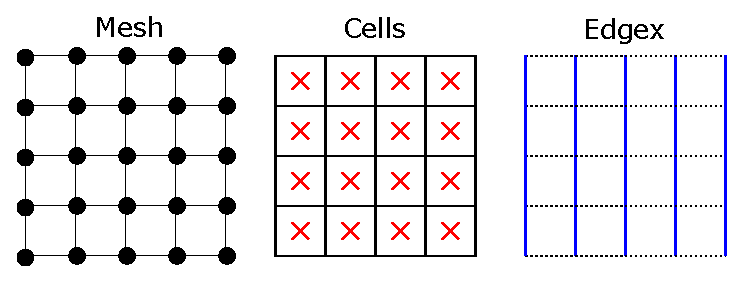
\includegraphics{./images/mesh.pdf}}
}
\hspace{10pt}
\subfloat[First stencil example\label{fig:ex1}]{
\resizebox{5cm}{!}{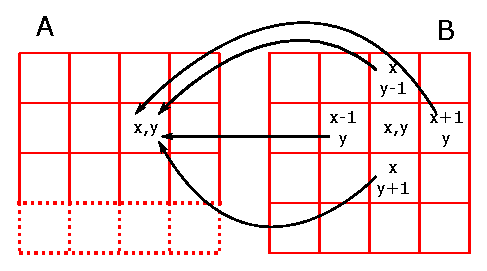
\includegraphics{./images/stencil1.pdf}}
}
\hspace{10pt}
\subfloat[Second stencil example\label{fig:ex2}]{
\resizebox{5cm}{!}{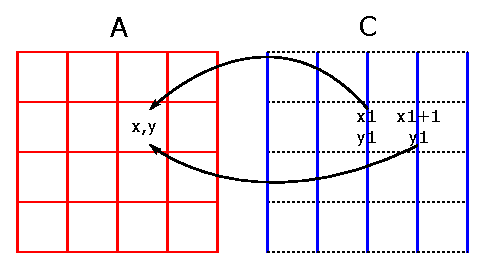
\includegraphics{./images/stencil2.pdf}}
}
\end{center}
\caption{Stencil examples}
\label{fig:gspmsp}
\end{figure}

% \begin{figure}[!h]\begin{center}
%   \resizebox{7cm}{!}{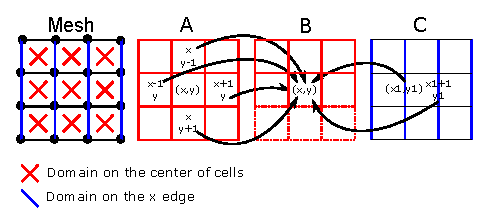
\includegraphics{./images/stencil.pdf}}
%   \caption{Examples of a stencil computations}
%   \label{fig:ex}
% \end{center}\end{figure}

The stencil computation in Figure~\ref{fig:ex1} computes $A$ using $B$, while the one in Figure~\ref{fig:ex2} computes $A$ using $C$. Thus, a stencil computation is defined by a set of input data (in those examples only one input data), and a single output data, the result. The \emph{computation domain} is a subset of elements to compute on the output data. In other words a computation domain is a subset of a mesh domain. For example, in the first stencil, the computation of $A$ is performed on plain elements, while dotted elements are not computed. On the other hand, on the second computation, the computation domain of $A$ is exactly equal to the cell mesh domain. The computation domain represents the set of elements on which the computation is performed, in other words, the space loop.

Finally, a stencil computation is composed of a \emph{numerical expression} which indicates how to compute an element of the computation domain (on the output data), using elements of the set of input data. The numerical expression of a stencil computation has the particularity to use not only the element to compute but also a \emph{neighborhood} of this element, also called a \emph{stencil shape}. For example, the stencil shape of the first computation in Figure~\ref{fig:ex1} contains direct neighbors on the right, left, top and bottom. Sometimes, the neighborhood shape can also access a different mesh domain, as for example in Figure~\ref{fig:ex2}. Actually, in this computation, the neighborhood contains edges on the left and on the right of a cell. As an example, the numerical expression of the first example could be:
\begin{equation*} 
A(x,y) = B(x+1,y)+B(x-1,y)+B(x,y+1)+B(x,y-1),
\end{equation*}
and the numerical expression of the second example could be:
\begin{equation*} 
A(x,y) = A(x,y)+C(x1,y1)+C(x1+1,y1).
\end{equation*}

%----------------------------------------
\subsection{A Multi-Stencil Formlization}
\label{sect:multistencil}
%----------------------------------------
A real case numerical simulation is most of the time composed of more than one stencil computation, with one or more stencil shapes, and onto one or more data, and of additionnal local computations.
\fix{cp2hc: [optionnelle] Par example? domaine applicatif?}
Let introduce some formal definitions used in the rest of the paper.

For $\Delta$ the set of data of the simulation, a stencil computation $s$ is defined as the quintuplet
\begin{equation} 
s(R,w,exp,d_c),
\label{eq:st}
\end{equation}
where $R$ is a set of pair $(r,n)$, with $r \in \Delta$ is a data read by the computation, and $n$ is a stencil shape (a neighborhood) applied on $r$. The data written by the computation is denoted $w \in \Delta$, $exp$ is the numerical expression of the stencil computation. Finally the numerical expression is applied on the computation domain $d_c$.

For example, in the example of Figure~\ref{fig:ex1}, assuming the computation domain (plain lines) is $dc1$ and the stencil shape is $n1$, the stencil computation can be defined with:
\begin{equation*}
R: {(B,n1)} \quad w: A \quad d_c: dc1
\end{equation*}
\begin{equation*}
exp: A(x,y)=B(x+1,y)+B(x-1,y)+B(x,y+1)+B(x,y-1).
\end{equation*}
On the other hand, in the example of Figure~\ref{fig:ex2}, assuming the computation domain is $dc2$ and the stencil shape is $n2$, the stencil computation can be defined with:
\begin{equation*}
R: {(C,n2),(A,null)} \quad w: A \quad d_c: dc2
\end{equation*}
\begin{equation*}
exp: A(x,y)=A(x,y)+C(x1,y1)+C(x1+1,y1)
\end{equation*}
One can notice that the input data $A$ is associated to the stencil shape $null$. This means that no stencil shape is applied on $A$, but only local accesses.

A local, or auxiliary, computation is almost the same than a stencil computation without neighborhood information in the numerical expression, which makes this kind of computation purely local. A local computation $l$ is defined as the quadruplet:
\begin{equation} 
l(R_l,w,exp,d_c),
\label{eq:loc}
\end{equation}
where $R_l$ is the set of input data, and other parameters are the same than for a stencil computation.

A multi-stencil program in this work is defined as a sextuplet:
\begin{equation} 
\mathcal{MSP}(T,\mathcal{M},\mathcal{D}_m,\mathcal{D}_c,\Delta,\Gamma),
\label{eq:msp}
\end{equation}
where $T$ is the set of time iteration to run the simulation, $\mathcal{M}$ is the mesh of the simulation, $\mathcal{D}_m$ is the set of mesh domains, $\mathcal{D}_c$ is the set of computation domains used into computations, $\Delta$ is the set of data of the simulation, each one mapped onto a mesh domain, and finally $\Gamma$ is the set of computations. The set of computations $\Gamma$ is composed of an ordered list of stencil and local computations. One can notice that this work is limited to a single type of mesh in a given simulation.

% !!!!!!!!!!!! a mettre en plus court autre part !!!!!!!!!!!!!!!
%----------------------------------------
% \subsection{Parallelization techniques}
% \label{sect:parallel}
%----------------------------------------
% Three classical parallelization techniques are used in this paper and are described in this section, the data parallelism, the task parallelism, and the hybrid data and task parallelism. Those parallelization techniques are independent from the actual parallel hardware used.

% \paragraph{Data parallelism} The idea of this parallelization technique is to split, or partition, data on which computations are applied among available processors (or cores). Each processor then applies the same progam or instruction onto its subpart of data. Moreover, if a neighborhood information is needed from another processor communications or synchronizations are performed. 

% In the domain of numerical simulations, this technique is most of the time called a domain decomposition. This parallelization technique produce efficient programs up to thousands processors or cores, but on certain conditions. First, each subpart of data has to be big enough to overlap communication time. Second, the partitioning of data has to be balanced among processors. Thus, if this parallelization technique is clearly adequate to structured meshes, easy to balance, it is not for unstructured meshes or irregular structures where the amount of work is not heterogenous.

% \paragraph{Task parallelism} Another well known parallelization technique is to identify in a program the different tasks and which one are independant and can be launched concurrently. Most of the time, such a prallelization technique create a dependency directed acyclic graph (dependency dag) from a set of ordered tasks. Dependencies are found from read/write information for each task. Actually, if a task $i$ write a data $a$ and if a task $j$ read $a$, then $i$ has to be finished before $j$ is performed. From a dependency graph two different solutions are available. First, a static schedule of tasks is built, which could be a good solution if the tasks are regular, or use a dynamic scheduler to dynamically decide at runtime which task is executed on which processor.

% \paragraph{Hybrid parallelism} Finally, it is also possible to combine both those parallelization techniques to get what is called an hybrid parallelization. The interest of an hybrid parallelization is to bring another source of parallelism if limits of a given technique are reach.


%----------------------------------------
\section{MSL and MSCAC Overview }
\label{sect:mscac}
The solution proposed in this paper contains a domain specific language to describe a multi-stencil program, i.e. an overall numerical simulation, and a compiler which successively parses the front-end language, transforms the internal representation, and finally dumps the representation to a back-end code. This back-end code is component based.

The proposed DSL, named MSL (\emph{Multi-Stencil Language}), is an agnostic descriptive language for multi-stencil simulations. Agnostic means that the description of a numerical simulation does not depend on implementation choices as, for example, the type of mesh (structured, unstructured), or its associated interfaces (how to define a stencil shape, etc.). Descriptive, on the other hand, means that the terminal states of the language grammar are (string) identifiers. As a result, MSL is not made to handle the expression of numerical computations, but only the description of a multi-stencil simulation, in a coarse-grain fashion. Numerical computations are encapsulated in specific components that users have to develop. In a MSL description, six main sections are defined, as the six tuples of the definition of a multi-stencil program $\mathcal{MSP}(T,\mathcal{M},\mathcal{D}_m,\mathcal{D}_c,\Delta,\Gamma)$ (\cf Equation~\ref{eq:msp}).

\begin{figure}[t]
\begin{center}
\begin{tikzpicture}[remember picture,
  inner/.style={rectangle,rounded corners=3pt,thick,inner sep=5pt},
  outer/.style={rectangle,rounded corners=3pt,thick,inner sep=5pt}
  ]
  \node (MSL) {MS Language};
  \node[outer,below=0.5 of MSL,draw=black] (MSCAC) {
    \begin{tikzpicture}
      \node [inner,draw=black,thick] (pars)  {Parser};
      \node [inner,draw=black,thick,below=0.5cm of pars] (MSC)  {MSC};
      \node [inner,below=0.5cm of MSC,draw=black,thick] (Dump)  {Dump};

      \draw[->] (pars) -- (MSC);
      \draw[->] (MSC) -- (Dump);
    \end{tikzpicture}
  };
  \node [below=0.5 of MSCAC] (CA) {Component Assembly};
  \node [rotate=90,above left=0.5 of MSC] (CAid) {MSCAC};
  \draw[->] (MSL) -- (pars.north);
  \draw[->] (Dump.south) -- (CA);
\end{tikzpicture}
\caption{The three phases of the MSCAC compiler.}
\label{fig:mscac}
\end{center}
\end{figure}

As illustrated in Figure~\ref{fig:mscac}, the compiler, named MSCAC for \emph{Multi-Stencil Component Assembly Compiler}, is composed of three different phases. The first phase of the compiler is to \emph{parse} the MSL description. Second, the compiler analyzes and transforms the computation part of the description $\Gamma$, to an intermediate representation. This phase of compilation, called MSC, is responsible for the automatic parallelization of the overall numerical simulation. Finally, the parallel intermediate representation is dumped to an actual implementation of the parallel pattern of the simulation.

% As illustrated in Figure~\ref{fig:mscac}, the MS language compiler, called MSCAC for \emph{Multi-Stencil Component Assembly Compiler}, is composed of two different parts. First, the computation compiler, called \emph{MSC}, is responsible for the parallelization of computations and for its dump to a component assembly; second, the data compiler, called \emph{MSD}, handles a distributed data structure, data mapped onto it, and their relations with computations, as a final overall component assembly.

%In this paper are presented the language MSL, the MSC compilation phase, and the dump compilation phase. 
The parallelization techniques handled by MSC are \emph{data parallelism}, where data are splitted among processors or cores while applying a single program everywhere, and \emph{task parallelism} where the program is transformed into a dependency graph of tasks. From a dependency graph, different strategies can be used to schedule tasks, in other words to control their execution in a valid order. The MSC compiler presented in this paper handles the transformation of the dependency graph to a static scheduling.

The final phase of compilation, the dump, uses the static schedule of the tasks, created from $\Gamma$, and additionnal information on $T$, $\mathcal{M}$, $\Delta$, $\mathcal{D}_m$ and $\mathcal{D}_c$, given by the \emph{parser}, to produce a back-end solution which represents the parallel pattern or skeleton of the overall simulation. We could have propose a dump to OpenMP~\cite{660313}, however this paper presents a first contribution to dump a DSL to a component-based runtime. Component models, where a component represents a clear and independent functionnality of the application, have first been proposed in software engineering and have proved many times good properties for code re-use, separation of concerns, maintainability and productivity of codes. Those properties, on the other hand, are recurrent stated problems of parallel applications.

The back-end of the compiler builds a component assembly, that can be divided in two parts: the components implementing the actual computation and the static schedule, and the components needed needed to manage it, \ie the runtime support. A general view of this assembly is proposed in Figure~\ref{fig:assembly}; it is explained in details in Section~\ref{sect:component}. As illustrated in the figure, each component is linked to one or more tuple of the multi-stencil program definition: \emph{DDS} component represents $\mathcal{M}$ and $\mathcal{D}_m$; \emph{Data} component represents $\Delta$ and $\mathcal{D}_c$; \emph{Time} component represents $T$, and \emph{Computations} component (which is generated by MSC) represents $\Gamma$.

The final back-end component assembly is a ready-to-fill parallel structure where the user has to write computation codes described in the MSL description. To write those computations, interfaces of the choosen implementation have to be used. For example, the back-end evaluated in this paper uses the distributed data structure proposed in SkelGIS library~\cite{CPE:CPE3494}. A work in progress replaces this DDS component by another one making using of Global Arrays~\cite{Nieplocha:2006:AAP:1125980.1125985}.

\begin{figure}[t]
\begin{center}
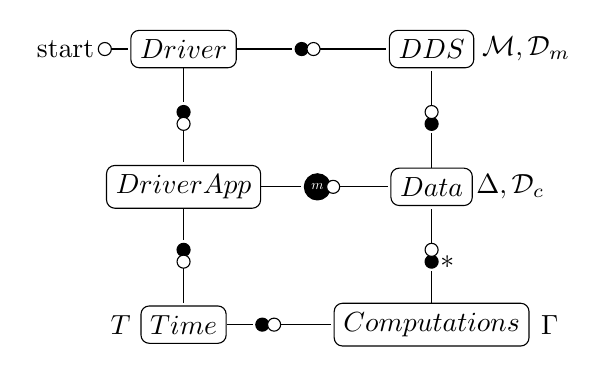
\begin{tikzpicture}[shorten >=1pt, node distance=2cm, on grid, auto]
   \node[component] (D) at (0,0) {$Driver$};
   \node[provide] (Dp) at (-1,0) {};
   \node (Ds) at (-1.5,0) {start};
   \node[use,right=1.5cm of D] (Du1) {};
   \node[use,below=0.8cm of D] (Du2) {};

   \node[provide,below=0.15 of Du2] (DAp) {};
   \node[component,below=0.8cm of DAp] (DA) {$DriverApp$};
   \node[use,right=1.7cm of DA] (DAu1) {$m$};
   \node[use,below=0.8cm of DA] (DAu2) {};

   \node[provide,below=0.15 of DAu2] (Tp) {};
   \node[component,below=0.8cm of Tp] (T) {$Time$};
   \node[use,right=1cm of T] (Tu) {};
   \node[left=0.8cm of T] (tt) {$T$};

   \node[provide,right=0.15 of Tu] (Cp) {};
   \node[component,right=2cm of Cp] (C) {$Computations$};
   \node[use,above=0.8cm of C] (Cu) {};
   \node[right=0.2cm of Cu] (star) {$*$};
   \node[right=1.5cm of C] (gamma) {$\Gamma$};

   \node[provide,right=0.2 of DAu1] (Datap1) {};
   \node[provide,above=0.15 of Cu] (Datap2) {};
   \node[component,above=0.8cm of Datap2] (Data) {$Data$};
   \node[use,above=0.8cm of Data] (Datau) {};
   \node[right=1cm of Data] (delta) {$\Delta,\mathcal{D}_c$};

   \node[provide,right=0.15 of Du1] (DDSp1) {};
   \node[provide,above=0.15 of Datau] (DDSp2) {};
   \node[component,above=0.8cm of DDSp2] (DDS) {$DDS$};
   \node[right=1.2cm of DDS] (m) {$\mathcal{M},\mathcal{D}_m$};
 
  \path[-]
    (Dp) edge node {} (D)
    (D) edge node {} (Du1)
        edge node {} (Du2)
    (DDSp1) edge node {} (DDS)
    (DA) edge node {} (DAu1)
           edge node {} (DAu2)
    (DAp) edge node {} (DA)
    (Tp) edge node {} (T)
    (T)  edge node {} (Tu)
    (Cp) edge node {} (C)
    (C) edge node {} (Cu)
    (Datap2) edge node {} (Data)
    (Datap1) edge node {} (Data)
    (Data) edge node {} (Datau)
    (DDSp2) edge node {} (DDS);
\end{tikzpicture}
\caption{Overall back-end component assembly}
\label{fig:assembly}
\end{center}
\end{figure}

% This paper presents the MS language and the MSC part of the compiler. The MSC compiler produces a static scheduling of the set of computations, ready to dump to a parallel language, such as OpenMP~\cite{660313} or HPF~\cite{219857}, but also ready to dump to a component assembly which is the main contribution of this work.

% \begin{figure*}
% \begin{center}
% \begin{tikzpicture}[shorten >=1pt, node distance=2cm, on grid, auto]
%    \node[component] (D) at (0,0) {$Driver$};
%    \node[provide] (Dp) at (-1,0) {};
%    \node (Ds) at (-1.5,0) {start};
%    \node[use] (Du1) at (1,0.5) {};
%    \node[use] (Du2) at (1,-0.5) {};

%    \node[component,right=1cm of Du2] (DA) {$DriverApp$};
%    \node[use] (DAu1) at (3.5,0) {$m$};
%    \node[use] (DAu2) at (3.5,-1) {};

%    \node[component] (T) at (4.5,-1) {$Time$};
%    \node[use,right=1cm of T] (Tu) {};
%    \node[component,right=2cm of Tu] (C) {$Computations$};
%    \node[use,right=2cm of C] (Cu) {};
%    \node[below=0.2cm of Cu] (star) {$*$};

%    \node[component,right=8cm of DAu1] (Data) {$Data$};
%    \node[use,right=1cm of Data] (Datau) {};

%    \node[component,right=13cm of Du1] (DDS) {$DDS$};
 
%   \path[-]
%     (Dp) edge node {} (D)
%     (D.east) edge node {} (Du1)
%       edge node {} (Du2)
%     (Du1) edge node {} (DDS.west)
%     (Du2) edge node {} (DA)
%     (DA.east) edge node {} (DAu1)
%       edge node {} (DAu2)
%     (DAu1) edge node {} (Data.west)
%     (DAu2) edge node {} (T)
%     (T) edge node {} (Tu)
%     (Tu) edge node {} (C)
%     (C) edge node {} (Cu)
%     (Cu) edge node {} (Data.west)
%     (Data) edge node {} (Datau)
%     (Datau) edge node {} (DDS.west);
% \end{tikzpicture}
% \caption{Shape of the generated component assembly.}
% \label{fig:assembly}
% \end{center}
% \end{figure*}

% It has to be noticed that in this paper, the MSD compiler is a first adhoc version which works for a precise distributed data structure, the SkelGIS library~\cite{HeleneLS13,HeleneLS14,HeleneEuroPar14,CPE:CPE3494}. However, using the system of python string templates~\footnote{\url{https://docs.python.org/2/library/string.html}} to define the component assembly part which manages data, it is already possible to use another distributed data structure, as for example Global Arrays~\cite{Nieplocha:2006:AAP:1125980.1125985}. This part of the compiler takes place in a larger research project to propose domain decomposition skeletons using component models.

% The overall compiler MSCAC produces a ready-to-fill component-based parallel structure of the simulation. In this final component assembly, it is needed to write computation components, using interfaces of the distributed data structure choosen by MSD. Thus, this work is complementary to stencil compilers or to distributed data structure solutions.

%----------------------------------------
%----------------------------------------
\subsection{Multi Stencil Language}
%----------------------------------------

\begin{filecontents*}{grammar.txt}
program ::= "mesh:" meshid 
            "mesh entities:" listmeshent
            "computation domains:" 
                       listcompdom
            "independent:"
                       listinde
            "data:" listdata
            "time:" iteration
            "computations:" listcomp
listmeshent ::= meshent listmeshent
             |  meshent
listcompdom ::= compdom listcompdom
             |  compdom
compdom ::= compdomid "in" listmeshent
listinde ::= inde listinde
          |  inde
inde ::= compdomid "and" compdomid
listdata ::= data listdata
          |  data
data ::= dataid "," meshent
iteration ::= num
listcomp ::= comp listcomp
          |  comp
comp ::= dataid "[" compdomid "]=" compid "(" 
            listdataread ")"
listdataread ::= dataread listdataread
              |  dataread
dataread ::= dataid "[" neighborid "]"
          |  dataid
\end{filecontents*}

\begin{filecontents*}{example.txt}
mesh: cart
mesh domains: cell,edgex,edgey
computation domains:
  allcell in cell
  alledgex in edgex
  alledgey in edgey
  part1edgex in edgex
  part2edgex in edgex
independent:
  part1edgex and part2edgex
data:
  a,cell
  b,cell
  c,edgex
  d,edgex
  e,edgey
  f,cell
  g,edgey
  h,edgex
  i,cell
  j,edgex
time:500
computations:
  b[allcell]=c0(a)
  c[alledgex]=c1(b[n1])
  d[alledgex]=c2(c)
  e[alledgey]=c3(c)
  f[allcell]=c4(d[n1])
  g[alledgey]=c5(e)
  h[alledgex]=c6(f)
  i[allcell]=c7(g,h)
  j[partedgex]=c8(i[n1])
\end{filecontents*}

\begin{figure*}[t]
\subfloat[\label{fig:grammar}]
{\lstinputlisting[basicstyle=\small,mathescape,frame=single,language=Python,numbers=left,linewidth=0.45\textwidth]{grammar.txt}}
%\hfill
\hspace{1.5cm}
\subfloat[\label{fig:mslex}]
{\lstinputlisting[basicstyle=\small,mathescape,frame=single,language=Python,numbers=left,linewidth=0.45\textwidth]{example.txt}}
\caption{(a) Grammar of the Multi-Stencil Language, (b) Example of a MSL program}
\end{figure*}

As mentioned in the previous section, the Multi Stencil Language (MSL) is an agnostic descriptive language for multi-stencil simulations. Six main sections are required in a MSL description that match the six elements of the formal definition; they describe: \textbf{1.}\,the mesh, \textbf{2.}\,the mesh entities, \textbf{3.}\,the computation domains with their inter-dependencies, \textbf{4.}\,the data, \textbf{5.}\,the time iterations, and finally \textbf{6.} the computations.
Figure~\ref{fig:grammar} shows the grammar of MSL. Lines 1 to 9 define what is a MSL program with the different parts mentioned above. The remaining of this section describes those different parts of a MSL program and presents an example.
One can notice that almost all terminals \texttt{meshid}, \texttt{meshdom}, \texttt{compdomid}, \texttt{dataid}, \texttt{compid} and \texttt{neighborid}, are string identifiers. Only \texttt{num} is an integer terminal.

\subsubsection*{Mesh and Mesh Entities}
As illustrated in the first line of the grammar in Figure~\ref{fig:grammar}, a mesh is simply defined by a string identifier.
The different kind of mesh entities are described as a list of identifiers (lines 2, 10 and 11 in Figure~\ref{fig:grammar}).
Figure~\ref{fig:mslex} presents an example of a mesh named \texttt{cart} used to represent a Cartesian mesh, and three kind of mesh entities: \texttt{cell}, \texttt{edgex}, and \texttt{edgey}.

\subsubsection*{Computation Domains and Their Dependencies}
A computation domain is a subset of a given kind of mesh entities, used during one or more computations.
For each computation domain, the kind of mesh entities on which it is mapped is specified (lines 3-4 and 12-14 on Figure~\ref{fig:grammar}).
By default, two computation domains of the same entities are handled as intersecting except when an explicit independence relation is mentioned in the \emph{independent} section of the language (lines 5-6 and 15-17 in Figure~\ref{fig:grammar}).
On lines 4 to 6 of Figure~\ref{fig:mslex}, computation domains are defined for each kind of mesh entities: \texttt{allcell}, \texttt{alledgex} and \texttt{alledgey}; they are used to represent the whole domain.
On lines 7 and 8 two other domains of \texttt{edgex} are defined: \texttt{part1edgex} and \texttt{part2edgex}; they are used to represent the boundaries of the domain.
On line 10 the independence relation between \texttt{part1edgex} and \texttt{part2edgex} is specified.

\subsubsection*{Data and Time}
A data element is a quantity to simulate. It is mapped on a given kind of mesh entities, as illustrated in lines 7 and 18-20 of Figure~\ref{fig:grammar}. The \texttt{time} section simply indicates a number of iterations to perform in the simulation. In the example of Figure~\ref{fig:mslex} ten data elements are defined and 500 iterations (lines 11-22). %An extension could be to support a convergence criterion.


\subsubsection*{Computation Description}
The last part of the language contains the specifications of stencil and local kernels as defined in Section~\ref{sect:multistencil}.
This description does not contain a direct expression of the numerical expressions $exp$.
Instead, the term $exp$ of Equations~\ref{eq:st} and~\ref{eq:loc} simply corresponds to an identifier that references an implementation in an external language  (\cf Section~\ref{sect:component}).
The specification starts by the identifier of the computed data element ($w$ in the formal description) with the computation domain between brackets ($d$).
Then, after the equal sign, the kernel identifier ($exp$) is specified.
Finally, between the parenthesis is the list of identifiers of the data elements read by the computation with their stencil shape between brackets ($R$).
If the computation is local, no brackets appear ($R_l$). In the example of Figure~\ref{fig:mslex}, nine computations are described. On line 24, the data element \texttt{b} is computed on the domain \texttt{allcell} by the kernel expression \texttt{c\_0} which read data \texttt{a} without neighborhood shape.

%----------------------------------------
\subsection{MSC Parallelization}
%----------------------------------------
The MSC parallelization is a subpart of the overall compiler MSCAC.
It makes use of the ordered list of computations $\Gamma$, which can directly be extracted from the parser, to build a parallel representation of the computations of the overall multi-stencil program.
This parallelization phase is divided in five different steps to transform $\Gamma$ to a series-parallel tree decomposition~\cite{Valdes:1979:RSP:800135.804393}.
%Data parallelism is handled in the first two steps, and task parallelism in the following three steps.
This section gives an overview of these five steps , but they are more formally defined with their associated algorithms in a research report~\cite{????}.

\subsubsection*{The Ordered List of Computations: $\Gamma$}
$\Gamma$ is directly obtained from the parser. Actually, the list of computations in the MSL program is already ordered: $\Gamma$ is a direct map of this list. In the example of Figure~\ref{fig:mslex}, $\Gamma = [c_0,c_1,c_2,c_3,c_4,c_5,c_6,c_7,c_8]$.

\subsubsection*{The Synchronized Ordered List of Computations: $\Gamma_{sync}$}
In a data parallelization, data is split among processors and the same program is applied on each sub-part of the data.
However, this parallelization technique requires additional synchronizations between processors.
For example, as a stencil kernel accesses neighbor values, values computed by another processor are needed and must be synchronized. 
The required synchronizations can be automatically computed from the ordered list of computations $\Gamma$.
A synchronization is needed each time a data read by a stencil computation has been written by a previous computation. In such a case, a computation is added before the stencil computation. This \emph{synchronization computation} reads the data to synchronize, and write the same data. The computation domain of such a synchronization computation encompasses the whole mesh entities on which the data is declared. As a result, $\Gamma$ is transformed to a synchronized ordered list of computations $\Gamma_{sync}$.
For example, in Figure~\ref{fig:mslex}, the stencil computation $c_1$ reads the data element $b$ which has been written by $c_0$. For this reason the sublist $[c_0,c_1]$ of $\Gamma$ is transformed into $[c_0,sync_1,c_1]$ in $\Gamma_{sync}$. The new computation $sync_1$ reads and writes $b$ and is applied on \texttt{edgex}. As a result, a dependency is kept between $c_0$ and $sync_1$ and between $sync_1$, and $c_1$. The same transformation is performed for all stencils: $c_4$ and $c_8$. Thus, $\Gamma_{sync} = [c_0,sync_1,c_1,c_2,c_3,sync_4,c_4,c_5,c_6,c_7,sync_8,c_8]$.

\subsubsection*{The Dependency Graph: $\Gamma_{dep}$}
From the synchronized ordered list of computations $\Gamma_{sync}$, a dependency graph $\Gamma_{dep}$ is built.
A dependency exists from computation $a$ to $b$ (including synchronizations) if and only if a data element read by $b$ has been written by $a$ in $\Gamma_{sync}$ with intersecting domains.
%In other words, the only case where the same data is manipulated by distinct kernels without inducing a dependency is when the computation domains do not intersect.
Nodes of the dependency graph represent computations of $\Gamma_{sync}$, while edges are dependencies between them. The dependency graph $\Gamma_{dep}$ is a directed acyclic graph (\emph{DAG}). For example, the dependency DAG $\Gamma_{dep}$ of the example of Figure~\ref{fig:mslex} is presented in Figure~\ref{fig:hyb}.

\begin{figure}[t]
\begin{center}
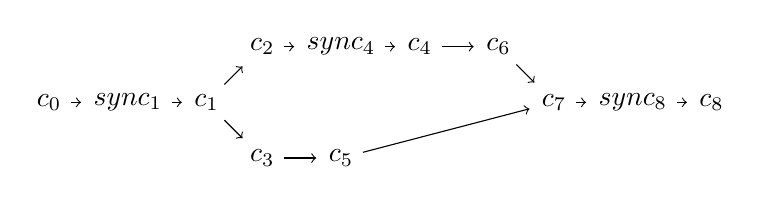
\begin{tikzpicture}[shorten >=1pt, node distance=2cm, on grid, auto]
   \node (c0) at (0,0) {$c_0$};
   \node[right=1 of c0] (sy1) {$sync_1$};
   \node[right=1 of sy1] (c1) {$c_1$};
   \node[above right=1 of c1] (c2) {$c_2$};
   \node[below right=1 of c1] (c3) {$c_3$};
   \node[right=1 of c2] (sy4) {$sync_4$};
   \node[right=1 of c3] (c5) {$c_5$};
   \node[right=1 of sy4] (c4) {$c_4$};
   \node[right=1 of c4] (c6) {$c_6$};
   \node[below right=1 of c6] (c7) {$c_7$};
   \node[right=1 of c7] (sy8) {$sync_8$};
   \node[right=1 of sy8] (c8) {$c_8$};
 
  \path[->]
    (c0) edge node {} (sy1)
    (sy1) edge node {} (c1)
    (c1)  edge node {} (c2)
          edge node {} (c3)
    (c2) edge node {} (sy4)
    (sy4) edge node {} (c4)
    (c4) edge node {} (c6)
    (c3) edge node {} (c5)
    (c5) edge node {} (c7)
    (c6) edge node {} (c7)
    (c7) edge node {} (sy8)
    (sy8) edge node {} (c8);
\end{tikzpicture}
\caption{$\Gamma_{hybrid}$ of the example of Figure~\ref{fig:mslex}}
\label{fig:hyb}
\end{center}
\end{figure}

\subsubsection*{The Minimal Series-Parallel Graph: $\Gamma_{msp}$}
Once a dependency graph is built, many solutions can be used to build a parallel application, as for example dynamic schedulers~\cite{Augonnet2011,Gautier:2013:XRS:2510661.2511383}. In this work a static scheduling of the dependency graph is built. To do so the dependency graph is transformed to a minimal series-parallel graph~\cite{Valdes:1979:RSP:800135.804393}. As it has been shown in~\cite{Valdes:1979:RSP:800135.804393}, the transitive reduction of a DAG is a minimal series-parallel graph if and only if a forbidden shape, called \emph{N-shape} and illustrated in Figure~\ref{fig:n}, is not found in the DAG. Thus, to transform $\Gamma_{dep}$ to the minimal series-parallel graph $\Gamma_{msp}$, an algorithm~\cite{Mitchell:2004:CMV:1082101.1082117} is applied to remove all \emph{N-shapes} by an over-constraint, as illustrated in Figure~\ref{fig:over}.

\begin{figure}[h!]
\begin{center}
\subfloat[][The forbidden $N$ shape.\label{fig:n}]{
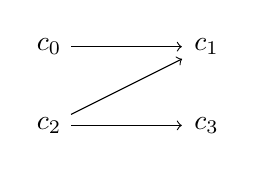
\begin{tikzpicture}[shorten >=1pt, node distance=2cm, on grid, auto]
   \node[] (a) at (0,0) {$c_0$};
   \node[] (b) at (2,0) {$c_1$};
   \node[] (c) at (0,-1) {$c_2$};
   \node[] (d) at (2,-1) {$c_3$};
 
  \path[->]
    (a) edge node {} (b)
    (c) edge node {} (b)
        edge node {} (d);
  \end{tikzpicture}
  }
  \hspace{25pt}
  \subfloat[][Over-constraint on the forbidden $N$ shape.\label{fig:over}]{
  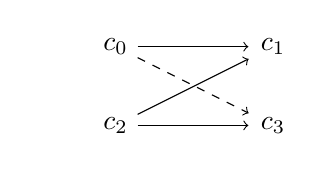
\begin{tikzpicture}[shorten >=1pt, node distance=2cm, on grid, auto]
   \node[] (c0) at (0,0) {$c_0$};
   \node[] (bc0) at (-1,0) {};
   \node[] (c1) at (2,0) {$c_1$};
   \node[] (c2) at (0,-1) {$c_2$};
   \node[] (bc2) at (-1,-1) {};
   \node[] (c3) at (2,-1) {$c_3$};
 
  \path[->]
    %(bc0) edge [dotted] node {} (c0)
    %(bc2) edge [dotted] node {} (c2)
    (c0) edge node {} (c1)
          edge [dashed] node [swap] {} (c3)
    (c2) edge node {} (c1)
        edge node {} (c3);
  \end{tikzpicture}
}
  \caption{Forbidden $N$ subgraph shape for a DAG to be minimal series-parallel.}
  \label{fig:forbidden}
\end{center}
\end{figure}

\subsubsection*{The Tree Decomposition: $\Gamma_{tsp}$}
Many works~\cite{Valdes:1979:RSP:800135.804393,Schoenmakers95anew} explains how to build a series-parallel tree decomposition from a minimal series-parallel graph. A series-parallel tree decomposition consists in the decomposition of the minimal series-parallel graph as a tree representing a set of \emph{sequences}, indicated by a $S$ node, and \emph{parallel} sections, indicated as a $P$ node. For example, the series-parallel tree decomposition $\Gamma_{tsp}$ of Figure~\ref{fig:hyb} is illustrated in Figure~\ref{fig:tsp}.

\begin{figure}[t]
\begin{center}
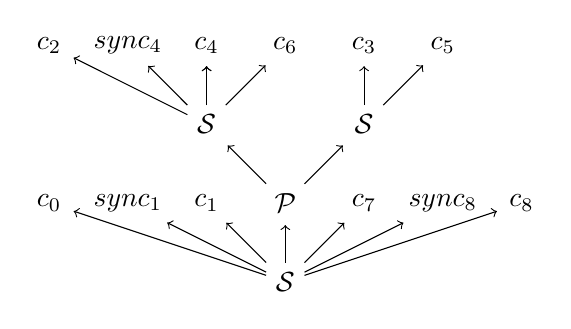
\begin{tikzpicture}[shorten >=1pt, node distance=2cm, on grid, auto]
   \node[] (s0)    at (0,0) {$\mathcal{S}$};
   
   \node[] (c0)    at (-3,1) {$c_0$};
   \node[] (star1) at (-2,1) {$sync_1$};
   \node[] (c1)    at (-1,1) {$c_1$};
   \node[] (p0)    at ( 0,1) {$\mathcal{P}$};
   \node[] (c7)    at ( 1,1) {$c_7$};
   \node[] (star8) at ( 2,1) {$sync_8$};
   \node[] (c8)    at ( 3,1) {$c_8$};

   \node[] (s1)    at (-1,2) {$\mathcal{S}$};
   \node[] (s2)    at (1,2) {$\mathcal{S}$};
   
   \node[] (c2)    at (-3,3) {$c_2$};
   \node[] (star4) at (-2,3) {$sync_4$};
   \node[] (c4)    at (-1,3) {$c_4$};
   \node[] (c6)    at ( 0,3) {$c_6$};
   \node[] (c3)    at ( 1,3) {$c_3$};
   \node[] (c5)    at ( 2,3) {$c_5$};

 
  \path[->]
    (s0) edge node {} (c0)
         edge node {} (star1)
         edge node {} (c1)
         edge node {} (p0)
         edge node {} (c7)
         edge node {} (star8)
         edge node {} (c8)
    (p0) edge node {} (s1)
         edge node {} (s2)
    (s1) edge node {} (c2)
         edge node {} (star4)
         edge node {} (c4)
         edge node {} (c4)
         edge node {} (c6)
    (s2) edge node {} (c3)
         edge node {} (c5);
  \end{tikzpicture}
\caption{$\Gamma_{tsp}$ of Figure~\ref{fig:hyb}. Nodes $S$ represent sequences, nodes $P$ represent parallel sections.}
\label{fig:tsp}
\end{center}
\end{figure}

\subsubsection*{Data parallelism optimizations: $\Gamma_{data}$}
Building the series-parallel tree decomposition $\Gamma_{tsp}$ is not only limited to the creation of a static scheduling of tasks. Actually, the tree can also be used to optimize the automatic generation of the data parallel structure of the simulation. In fact, creating a data parallelization of the simulation, it first seems natural to create the parallel structure directly from $\Gamma_{sync}$, as the program is parallelized from data decomposition and applying the same sequential algorithm on each processor. However, as a computation kernel in MSL writes a single data $w$ at a time (in order to entirely manage and order the dependencies between tasks), the same computation domain might be iterated more than once to compute different numerical expressions, while those expressions could be computed inside a single space loop. For this reason, an optimized and \emph{fusionned} ordered list of computation $\Gamma_{data}$ is built from $\Gamma_{tsp}$. Actually, in $\Gamma_{tsp}$, computations of a parallel subtree with a same computation domain can be computed in the same space loop, in any order. Moreover, in $\Gamma_{tsp}$, two consecutive computations of a sequence subtree with a same computation domain can be computed in the same space loop, if the order of computation of the sequence is kept.

% \paragraph{Dump to a component assembly} Finally, from the series-parallel tree decomposition $\Gamma_{tsp}$ we could build a program using any parallel language containing \emph{parallel sections} and \emph{sequences of instructions} such as OpenMP~\cite{660313}, HPF~\cite{219857}, UPC~\cite{El-Ghazawi:2006:UUP:1188455.1188483} etc. In this paper we study the dump of $\Gamma_{tsp}$ to a component assembly which needs the introduction of \emph{control components}, described in the next section.



%----------------------------------------
\section{A Component based Back-End}
\label{sect:component}
%----------------------------------------
%\subsection{Overview}
%----------------------------------------
This section describes both the projection of $\Gamma_{tsp}$ to
components, and the remaining needed components to execute a
multi-stencil application. Before those details the section gives an overview of
component models, and introduce the concepts of the Low Level Component Model \llc, which is used in this paper.


%----------------------------------------
\subsection{Component Model Overview}
%----------------------------------------
Component model is a domain of software
engineering~\cite{Szyperski:2002:CSB:515228}, which promotes code
re-use, separations of concerns, and thus maintainability. An
application is made of a set of components; a component being a kind of
black box representing an independent functionnality of the application, and which interacts only through its ports. A port specifies the services provided and required by the component.
%
With respect to high performance computing, some works have also shown
that component models can achieve the needed level of performance, and
scalability while also helping in application
portability~\cite{Bernholdt01052006, bigot:inria-00388508, UCHPC2015}

Many component models exist, each of them with its own specifications
and singularities. In distributed computing, well known component
models are CCM~\cite{corba:omg06} (CORBA Component Model), and
GCM~\cite{Baude} (Grid Component Model); in HPC, there are
CCA~\cite{Bernholdt01052006} (Common Component Architecture), and
\llc~\cite{l2c} (Low Level Component), for example.
%
As this work makes use of \llc, in particular for the experiments, let
introduce concepts of this component model with more details.

%----------------------------------------
\subsection{\llc}
%----------------------------------------

\llc is a minimalist \texttt{C++} based HPC-oriented component model
where a component extends the concept of class by specifying in its
interfaces the services that it offers ($provide$ ports) and that it
needs, either a single service instance ($use$ ports), or multiple
service instances ($use-multiple$ ports). Services are \texttt{C++}
interfaces. \llc also offers $MPI$ ports that enable components to
share MPI communicators. Components can also have attribute ports to
be configured.
%
As illustrated in Figures~\ref{fig:ports}, a $provide$ port is
represented with a white circle, a $use$
port with a black circle, a $use-multiple$ port by a black circle with
a white $m$ in it. MPI port are
connected with a black rectangle.

A classical \llc-based application is a static \emph{assembly} of
components made of instances of components and of connections between
component ports. Such an assembly is described in LAD, an XML
dialect~\cite{l2c}.

\begin{figure}[t]
\begin{center}
\subfloat[][\label{fig:2comp}]{
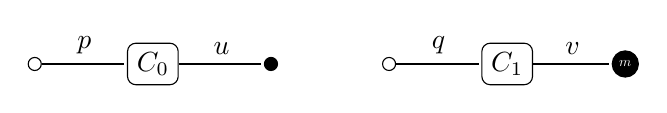
\begin{tikzpicture}[shorten >=1pt, node distance=2cm, on grid, auto]
   \node[component] (C) at (0,0) {$C_0$};
   \node[provide] (p) at (-1.5,0) {};
   \node[use] (u) at (1.5,0) {};
   \node[provide,right=1.5cm of u] (p1) {};
   \node[component,right=1.5cm of p1] (C1) {$C_1$};
   \node[use,right=1.5cm of C1] (um) {$m$};
 
  \path[-]
    (p) edge node {$p$} (C)
    (C.east) edge node {$u$} (u)
    (C1)  edge node {$v$} (um)
    (p1) edge node {$q$} (C1);
\end{tikzpicture}
}
\subfloat[][\label{fig:ass}]{
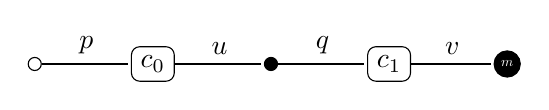
\begin{tikzpicture}[shorten >=1pt, node distance=2cm, on grid, auto]
   \node[component] (C) at (0,0) {$c_0$};
   \node[provide] (p) at (-1.5,0) {};
   \node[use] (u) at (1.5,0) {};
   \node[component,right=1.5 of u] (C1) {$c_1$};
   \node[use,right=1.5 of C1] (um) {$m$};
 
  \path[-]
    (p) edge node {$p$} (C)
    (C) edge node {$u$} (u)
    (C1)  edge node {$v$} (um)
    (u) edge node {$q$} (C1);
\end{tikzpicture}
}
\subfloat[][\label{fig:mpi}]{
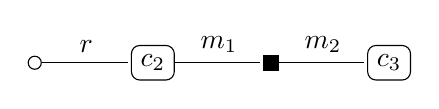
\begin{tikzpicture}[shorten >=1pt, node distance=2cm, on grid, auto]
   \node[component] (C) at (0,0) {$c_2$};
   \node[provide] (p) at (-1.5,0) {};
   \node[mpi] (u) at (1.5,0) {};
   \node[component,right=1.5 of u] (C1) {$c_3$};
 
  \path[-]
    (p) edge node {$r$} (C)
    (C) edge node {$m_1$} (u)
    (u) edge node {$m_2$} (C1);
\end{tikzpicture}
}
\caption{Example of components and their ports representation. a) Component $c_0$ has a provide port ($p$) and a use port ($u$); Component $c_1$ has also a provide port ($q$) but also a use multiple port ($v$). b) A use port is connected to a (compatible) provide port. c) Component $c_2$ and $c_3$ shares an MPI communicator.}
\label{fig:ports}
\end{center}
\end{figure}

%% In the rest of this paper, when a required service of a \emph{use} (or \emph{use-multiple}) port is filled and linked to a \emph{provide} port in the comonent assembly, only the use port stay visible, as illustrated in Figure~\ref{fig:assembly}. As the use port is on the right of its component, and the provide port on the left, in a component assembly the component on the left uses the provide port of the component on the right.

%----------------------------------------
\subsection{MSCAC Runtime Overview}
%----------------------------------------

Figure~\ref{fig:mscac:assembly} gives an overview of the back-end component
assembly that is executed. As discusses in Section~\ref{sect:mscac},
there are different types of components. Components~\texttt{Driver},
\texttt{DriverApp}, and \texttt{Time} are always instanciated in the final component assembly; the input MSL file is not used by them except the component \texttt{Time} which uses the terminal \texttt{iteration} of the grammar. There is also a
single Component~\texttt{DDS} (the current version handles a single mesh
type). All these components are provided with the
compiler; dumping this part of the assembly is straightforward.

While Component~\texttt{DDS} is managing the structure of the mesh,
each data of the simulation is handled by a component of type
\texttt{Data}. Therefore, the compiler generates in the assembly as
many instances of such component as needed, from the \texttt{data}
section of an MSL program.

The last part of the assembly is the computation part. Each computation kernel is embedded in a kernel component, denoted K, which have to be written by the user and provided
to the compiler. A kernel component encapsulates a computations. To
access data, a kernel component is connected, by the compiler, to the adequate
\texttt{Data} components such that their ports name respect the names
given in the \texttt{data} section of MSL. We denote the fact that they may have
several use port by adding a star on the use port, as illustrated in Figure~\ref{fig:k}.
\begin{figure}
\begin{center}
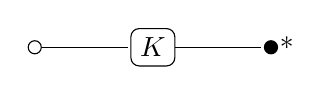
\begin{tikzpicture}[shorten >=1pt, node distance=2cm, on grid, auto]
   \node[component] (k) at (0,0) {$K$};
   \node[provide] (p) at (-1.5,0) {};
   \node[use] (u) at (1.5,0) {};
   \node[right=0.2 of u] (star) {*};
 
  \path[-]
    (p) edge node {} (k)
    (k) edge node {} (u);
\end{tikzpicture}
\end{center}
\caption{Kernel component.}
\label{fig:k}
\end{figure}
  
%% In the computation part of the simulation a final component is needed,
%% the computation component, denoted K. This type of component
%% represents a single computation of the simulation, i.e. the
%% computation of a single output data (written) using a set of input
%% data (read). Using a \emph{use-multiple}, however, a list of component
%% is used and the explicit identification of each component to use is
%% lost. If for SEQ or PAR, the identification of components is not
%% usefull, it is usefull to manipulate data in a computation. For this
%% reason a computation component has as much \emph{use} ports as input
%% and output data to manipulate. We denote this in the bellow
%% representation as a star on the use port.

The rest of the computation part of the assembly contains the static parallel schedule
computed by MSC, \ie $\Gamma_{tsp}$. This is achieved through the use of
three specific components which manage the $P$, $S$, and $sync$
operations of $\Gamma_{tsp}$ as explained hereafter.

%----------------------------------------
\subsection{Control Components}
%----------------------------------------
The series-parallel tree decomposition $\Gamma_{tsp}$ represents the
control of the dependencies of the simulation. As a result to be able
to dump it to a component assembly it is needed to introduce what can
be called \emph{control components}. Those components can be used for
any case of simulation which increases code reuse between
simulations. A control component is composed of a single
\emph{provide} port linked to a single execution method, most of the
time called the \emph{go} method. We introduce three types of control
components represented in Figure~\ref{fig:ctrlcomponents}.

\begin{figure}[t]
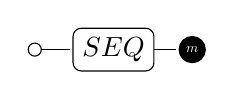
\begin{tikzpicture}[shorten >=1pt, node distance=1cm, on grid, auto]
   \node[component] (seq) at (0,0) {$SEQ$}; \node[provide] (p) at
   (-1,0) {}; \node[use] (u) at (1,0) {$m$};
 
  \path[-]
    (p) edge node {} (seq)
    (seq) edge node {} (u);
\end{tikzpicture}
\hspace{\fill}
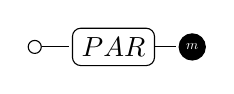
\begin{tikzpicture}[shorten >=1pt, node distance=1cm, on grid, auto]
   \node[component] (seq) at (0,0) {$PAR$};
   \node[provide] (p) at (-1,0) {};
   \node[use] (u) at (1,0) {$m$};
 
  \path[-]
    (p) edge node {} (seq)
    (seq) edge node {} (u);
\end{tikzpicture}
\hspace{\fill}
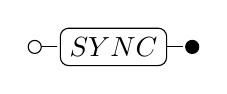
\begin{tikzpicture}[shorten >=1pt, node distance=1cm, on grid, auto]
   \node[component] (sync) at (0,0) {$SYNC$};
   \node[provide] (p) at (-1,0) {};
   \node[use] (u) at (1,0) {};
 
  \path[-]
    (p) edge node {} (sync)
    (sync) edge node {} (u);
\end{tikzpicture}
\\
a) Comp. SEQ
\hspace{\fill}
b) Comp. PAR
\hspace{\fill}
c) Comp. SYNC
\\
\caption{The three control components used by the back-end.}
\label{fig:ctrlcomponents}
\end{figure}

\begin{description}
\item[Sequence component (SEQ)] It is the direct representation of a sequence node of $\Gamma_{tsp}$. The role of this component is to call an ordered list of other components. Its interface contains an ordered \emph{use-multiple} port to be connected to the components to call in sequence.

\item[Parallel component (PAR)] It is the direct representation of a parallel node of $\Gamma_{tsp}$. The role of this component is to call simultaneously a set of other components. It offers a \emph{use-multiple} port to be connected to the components to call in parallel.
  
\item[Synchronization component (SYNC)]. It is the direct representation to an update leaf of $\Gamma_{tsp}$. The role of this component is to call the synchronization of a given data. It offers a \emph{use} port to be connected to the data to update.

\end{description}


%----------------------------------------
\subsection{Dump To Component Assembly}
%----------------------------------------
From $\Gamma_{tsp}$ and using the control components described above,
a direct dump can be done to a component assembly for an hybrid (data
and task) parallelization of a simulation. 
\fix{HC: ce qui suit est a changer avec la fusion du code de plusieurs composants}
However, it is also
possible to dump to a data parallelization only. In such a case the
computation of $\Gamma_{sync}$ is enough to generate the component
assembly. Actually a single SEQ component is thus needed and this
component is linked to all computations and synchronizations of
$\Gamma_{sync}$ directly.

Figure~\ref{fig:tsp:assembly} displays the assembly part corresponding to
$\Gamma_{tsp}$ of Figure~\ref{fig:tsp}. In this figure, the ports
linked to data (use and use-multiple ports of SYNC and K) are
represented but are not connected. Moreover, each computation
component is an instance of the component K presented before but using
the identification name of the computation in the MSL file.

\begin{figure*}[t]
\begin{center}
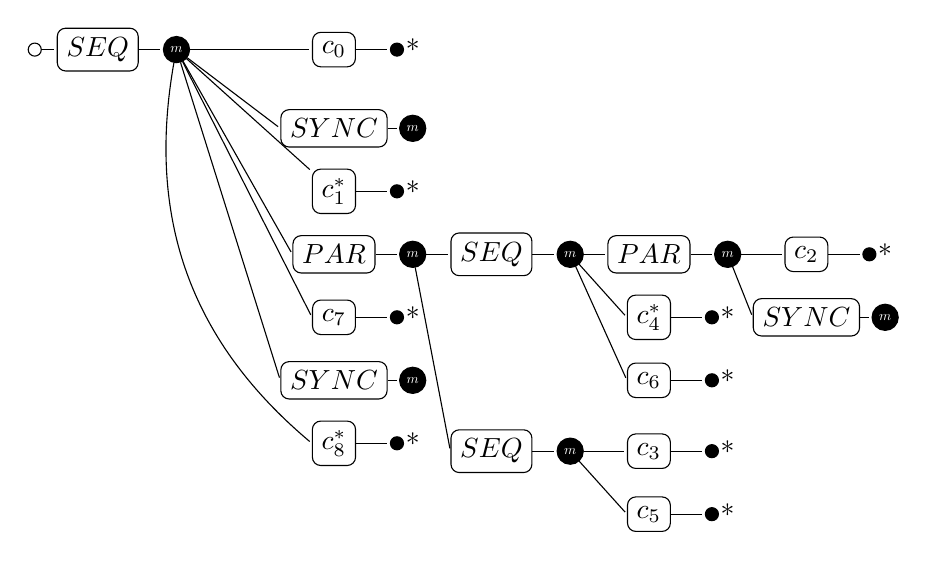
\begin{tikzpicture}[shorten >=1pt, node distance=2cm, on grid, auto]
   %seq0
   \node[component] (seq0) at (0,0) {$SEQ$};
   \node[provide] (seq0p) [left = 0.8cm of seq0] {};
   \node[use] (seq0u) [right = 1cm of seq0] {$m$};
   %c0
   \node[component] (c0) [right = 2cm of seq0u] {$c_0$};
   \node[use] (c0u) [right = 0.8cm of c0] {};
   \node[right=0.2 of c0u] (star) {*};
   %sync0
   \node[component] (sync0) [below = 1cm of c0] {$SYNC$};
   \node[use] (sync0u) [right = 1cm of sync0] {$m$};
   %c1
   \node[component] (c1) [below = 0.8cm of sync0] {$c_1^*$};
   \node[use] (c1u) [right = 0.8cm of c1] {};
   \node[right=0.2 of c1u] (star) {*};
   %par0
   \node[component] (par0) [below = 0.8cm of c1] {$PAR$};
   \node[use] (par0u) [right = 1cm of par0] {$m$};
  %seq1
   \node[component] (seq1) [right = 1cm of par0u] {$SEQ$};
   \node[use] (seq1u) [right = 1cm of seq1] {$m$};
   %par1
   \node[component] (par1) [right = 1cm of seq1u] {$PAR$};
   \node[use] (par1u) [right = 1cm of par1] {$m$};
  %c2
   \node[component] (c2) [right = 1cm of par1u] {$c_2$};
   \node[use] (c2u) [right = 0.8cm of c2] {};
   \node[right=0.2 of c2u] (star) {*};
  %sync1
   \node[component] (sync1) [below = 0.8cm of c2] {$SYNC$};
   \node[use] (sync1u) [right = 1cm of sync1] {$m$};
  %c4
   \node[component] (c4) [below = 0.8cm of par1] {$c_4^*$};
   \node[use] (c4u) [right = 0.8cm of c4] {};
   \node[right=0.2 of c4u] (star) {*};
  %c6
   \node[component] (c6) [below = 0.8cm of c4] {$c_6$};
   \node[use] (c6u) [right = 0.8cm of c6] {};
   \node[right=0.2 of c6u] (star) {*};
  %seq2
   \node[component] (seq2) [below = 2.5cm of seq1] {$SEQ$};
   \node[use] (seq2u) [right = 1cm of seq2] {$m$};
  %c3
   \node[component] (c3) [right = 1cm of seq2u] {$c_3$};
   \node[use] (c3u) [right = 0.8cm of c3] {};
   \node[right=0.2 of c3u] (star) {*};
  %c5
   \node[component] (c5) [below = 0.8cm of c3] {$c_5$};
   \node[use] (c5u) [right = 0.8cm of c5] {};
   \node[right=0.2 of c5u] (star) {*};
  %c7
   \node[component] (c7) [below = 0.8cm of par0] {$c_7$};
   \node[use] (c7u) [right = 0.8cm of c7] {};
   \node[right=0.2 of c7u] (star) {*};
  %sync2
   \node[component] (sync2) [below = 0.8cm of c7] {$SYNC$};
   \node[use] (sync2u) [right = 1cm of sync2] {$m$};
  %c8
   \node[component] (c8) [below = 0.8cm of sync2] {$c_8^*$};
   \node[use] (c8u) [right = 0.8cm of c8] {};
   \node[right=0.2 of c8u] (star) {*};

   \path[-]
   %seq0
    (seq0) edge node {} (seq0u)
    (seq0p) edge node {} (seq0)
   %c0
    (seq0u) edge node {} (c0)
    (c0) edge node {} (c0u)
    %sync0
    (seq0u) edge node {} (sync0.west)
    (sync0) edge node {} (sync0u)
    %c1
    (seq0u) edge node {} (c1)
    (c1) edge node {} (c1u)
   %par0
    (seq0u) edge node {} (par0.west)
    (par0) edge node {} (par0u)
  %seq1
    (par0u) edge node {} (seq1)
    (seq1) edge node {} (seq1u)
  %par1
    (seq1u) edge node {} (par1.west)
    (par1) edge node {} (par1u)
  %c2
    (par1u) edge node {} (c2)
    (c2) edge node {} (c2u)
  %sync0
    (par1u) edge node {} (sync1.west)
    (sync1) edge node {} (sync1u)
  %c4
    (seq1u) edge node {} (c4.west)
    (c4) edge node {} (c4u)
  %c6
    (seq1u) edge node {} (c6.west)
    (c6) edge node {} (c6u)
  %seq2
    (par0u) edge node {} (seq2.west)
    (seq2) edge node {} (seq2u)
  %c3
    (seq2u) edge node {} (c3)
    (c3) edge node {} (c3u)
  %c6
    (seq2u) edge node {} (c5.west)
    (c5) edge node {} (c5u)
  %c6
    (seq0u) edge node {} (c7.west)
    (c7) edge node {} (c7u)
  %sync2
    (seq0u) edge node {} (sync2.west)
    (sync2) edge node {} (sync2u)
  %c8
    (seq0u) edge [bend right] node {} (c8.west)
    (c8) edge node {} (c8u)
   ;
\end{tikzpicture}
\caption{Component assembly representing the computation part generated from $\Gamma_{tsp}$ of Figure~\ref{fig:tsp}.}
\label{fig:tsp:assembly}
\end{center}
\end{figure*}

%----------------------------------------

%----------------------------------------
\section{Real-case Evaluation}
\label{sect:eval}
This section evaluates the MSL compiler and the code it generates.
We first evaluate the generated code in the case where only data parallelization and fusion are applied and compare this to a full SkelGIS program.
Then, we analyze a case taking advantage of the full the hybrid parallelization combining data and task parallelism and validate the performance model proposed in Section~\ref{sect:tsp}.

All evaluations presented in this section are based on a real case study of the shallow-Water Equations as solved in  the FullSWOF2D\footnote{\url{http://www.univ-orleans.fr/mapmo/soft/FullSWOF/}}~\cite{Ferrari2004,CPE:CPE3494} code from the MAPMO laboratory, University of Orl\'eans.
We have developed a MSL version of FullSWOF2D that contains 3~mesh entities, 7~computation domains, 48~data and 98~computations (32~stencil kernels and 66~local kernels).

%-------------------------------------
\subsection{Compiler}

Table~\ref{fig:exectime} illustrates the execution time for each step of the MSL compiler for the FullSWOF2D example.
This has been computed on a laptop with a bi-core Intel Core i5 1.4~GHz, and 8~GB of DDR3.
While the overall time of 4.6 seconds remains reasonable, one can notice that the computation of the $TSP$ tree is by far the longest step of the compiler.
As a matter of fact, the complexity of the algorithm for N-shapes removal is $O(n^3)$.
The replacement of the static scheduling by a direct scheduling of the DAG by dedicated tools should solve this in the future.

\begin{table}[!h]
 \begin{center}
 \begin{tabular}{|c|c|c|c|c|}
  \hline
   Step & Parser & $\Gamma_{sync}$ & $\Gamma_{dep}$ & $TSP$\\
   \hline
   Time (ms) & 1 & 2 & 4.2 & 3998.5\\
   \hline
   \% & 0.022 & 0.043 & 0.09 & 86.6\\
   \hline
 \end{tabular}
\caption{Execution times of the MSL compiler}
\label{fig:exectime}
 \end{center}
\end{table}

%-------------------------------------
\subsection{Data parallelism}

The first parallelization technique proposed by MSL is a data parallelization. To implement this parallelization, the dump step of the MSL compiler uses the SkelGIS language. This language, as already described, offers a distributed Cartesian mesh and programming interfaces to use it as a sequential data structure. It has been evaluated itself compared to an MPI implementation on the same FullSWOF2D simulation~\cite{CPE:CPE3494}. What MSL brings to SkelGIS is an automatic detection of where MPI synchronizations are needed during the numerical simulation, and how to make a fusion of some computations in order to reduce cache misses. This section gives a performance comparison of the code produced by MSL for FullSWOF2D, and of the equivalent manual SkelGIS program (with manual synchronizations and fusion choices). Moreover, as the code produced by MSL is a component-based code, this evaluation also shows that no overheads are introduced \llc~\cite{l2c}. Following evaluations have been performed onto the machine of the TGCC Curie described in Table~\ref{tab:TGCC}. Each evaluation has been performed ten times and the median is presented in results.

\begin{table}[!h]
\begin{center}
 \begin{tabular}{|c|c|}
   \hline
    Cluster & \textbf{TGCC Curie Thin Nodes}\\
     \hline         
    Processor & 2$\times$SandyBridge\\
    & (2.7 GHz)\\
    Cores/node & 16 \\
    RAM/node & 64 GB\\
    RAM/core & 4GB\\
    Compiler [-O3] & gcc 4.9.1\\
    MPI & Bullxmpi\\
    Network & Infiniband\\
    \hline
 \end{tabular}
 \caption{\label{tab:TGCC}Hardware configuration of TGCC Curie Thin nodes.}
 \end{center}
\end{table}

\paragraph{\textbf{Weak scaling}} The first evaluation is a weak scaling evaluation. In a weak scaling, a constant amount of work is given to each core while increasing the overall number of cores. As a result, the overall domain size also increase with the number of cores. A weak scaling is a good evaluation to detect overheads which are independent from the amount of computation performed by each core, such as collective communications, or overheads introduced by \llc components, for example. Figures~\ref{fig:weak1} and~\ref{fig:weak2} respectively show the weak scaling evaluations for a $400 \times 400$ and a $800 \times 800$ domain for each core, from 16 cores to 16.384 cores. Minimum and maximum values are also shown as error bars in figures.

\begin{figure}[!h]\begin{center}
  \resizebox{8cm}{!}{\includegraphics{../results/weak_scaling/400/median_weak.pdf}}
  \caption{weak-scaling with $400 \times 400$ domain per core.}
  \label{fig:weak1}
\end{center}\end{figure}
\begin{figure}[!h]\begin{center}
  \resizebox{8cm}{!}{\includegraphics{../results/weak_scaling/800/median_weak.pdf}}
  \caption{weak-scaling with $800 \times 800$ domain per core.}
  \label{fig:weak2}
\end{center}\end{figure}

One can notice that the MSL code produces a better execution time on the $400 \times 400$ domain, while it produces a small overhead on the $800 \times 800$ domain. Those results could be due to different optimizations of the gcc compiler due to components. Actually, a component in \llc is compiled independently, as an dynamic library, with the \emph{-fpic} compilation option, while the SkelGIS version is compiled entirely as a single code. However, one can also notice that except those not significant differences of execution times, weak scalings have the same behavior on both codes.

\paragraph{\textbf{Strong scaling}} The second evaluation is a strong scaling evaluation. Unlike a weak scaling, a strong scaling keeps a constant overall size of problem, while the number of cores increase. As a result, the sub-domain computed by each core reduces while the number of cores increases. The strong scaling is a good additional evaluation to the weak scaling, showing different kinds of overheads, such as cache misses (when the size of sub-domain becomes small enough to fit into cache memory), or small constant overheads. Figure~\ref{fig:strong} shows the strong scaling evaluation for a $10k \times 10k$ overall domain size, from 16 cores to 16.384 cores. This strong scaling is illustrated with the number of iterations per seconds as a function of the number of cores. The ideal strong scaling is also illustrated.

\begin{figure}[!h]\begin{center}
  \resizebox{8cm}{!}{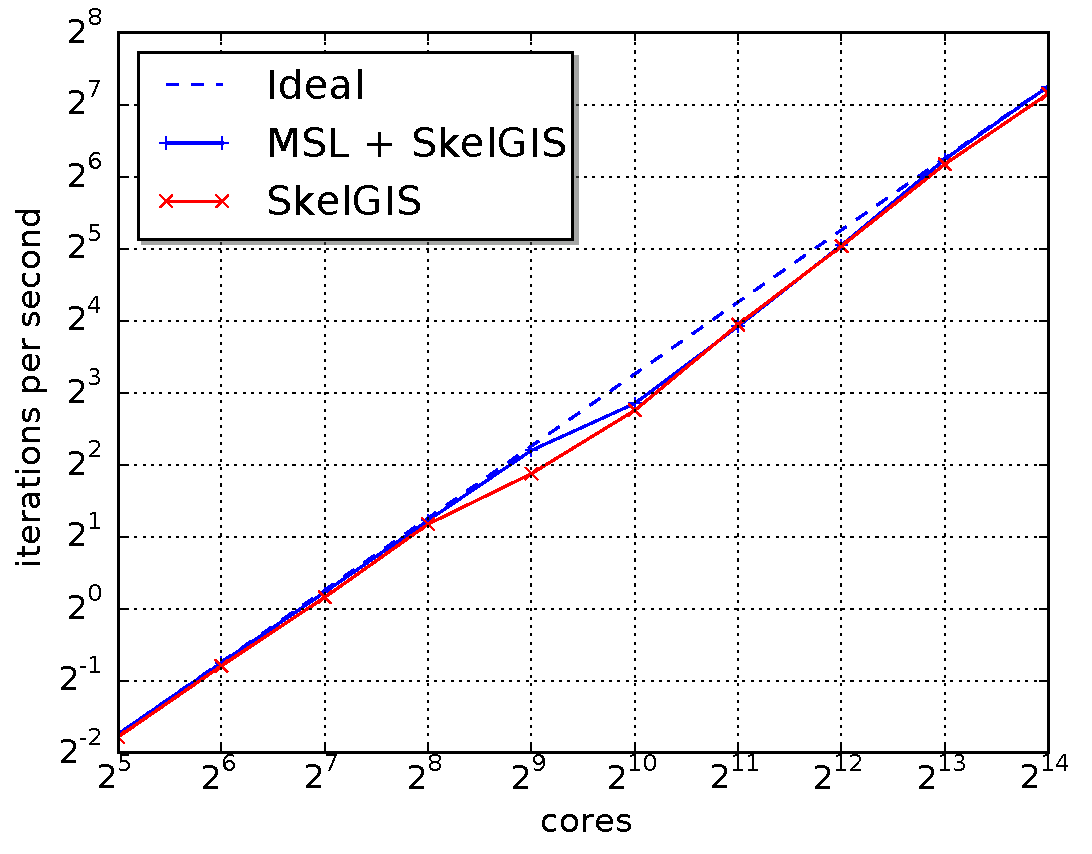
\includegraphics{../results/strong_scaling/10K_1K/median_strong.pdf}}
  \caption{Strong scaling on a $10k \times 10k$ domain.}
  \label{fig:strong}
\end{center}\end{figure}

First, one can notice that the strong scaling evaluated for the code generated by MSL is close to the ideal speedup up to 16.384 cores, which is a very good result. Moreover, no overheads are introduced by MSL which shows that automatic synchronization detections and automatic fusion detections are the same one that the one written manually into the SkelGIS code of FullSWOF2D. Finally, no overheads are introduced by components of \llc. A small behavior difference can be noticed with $2^9=512$ cores, however this variation is no longer observed with 1024 cores.

\paragraph{\textbf{Fusion}} Finally, to evaluate the data parallelization technique automatically introduced by MSL, the fusion optimization is evaluated. Figure~\ref{fig:fusion} shows the number of iterations per second as a function of the number of cores, for FullSWOF2D with and without fusion optimization and onto a $500 \time 500$ domain. As explained in Section~\ref{sect:fusion}, the MSL fusion happens at a high level and is most of the time done naturally by a computer scientist. However, for a non computer scientist which write its numerical codes, an automatic proposition of such fusions makes the implementation easier. Moreover, one can notice that the performance is clearly improved (around 40\%) by this fusion.

\begin{figure}[!h]\begin{center}
  \resizebox{8cm}{!}{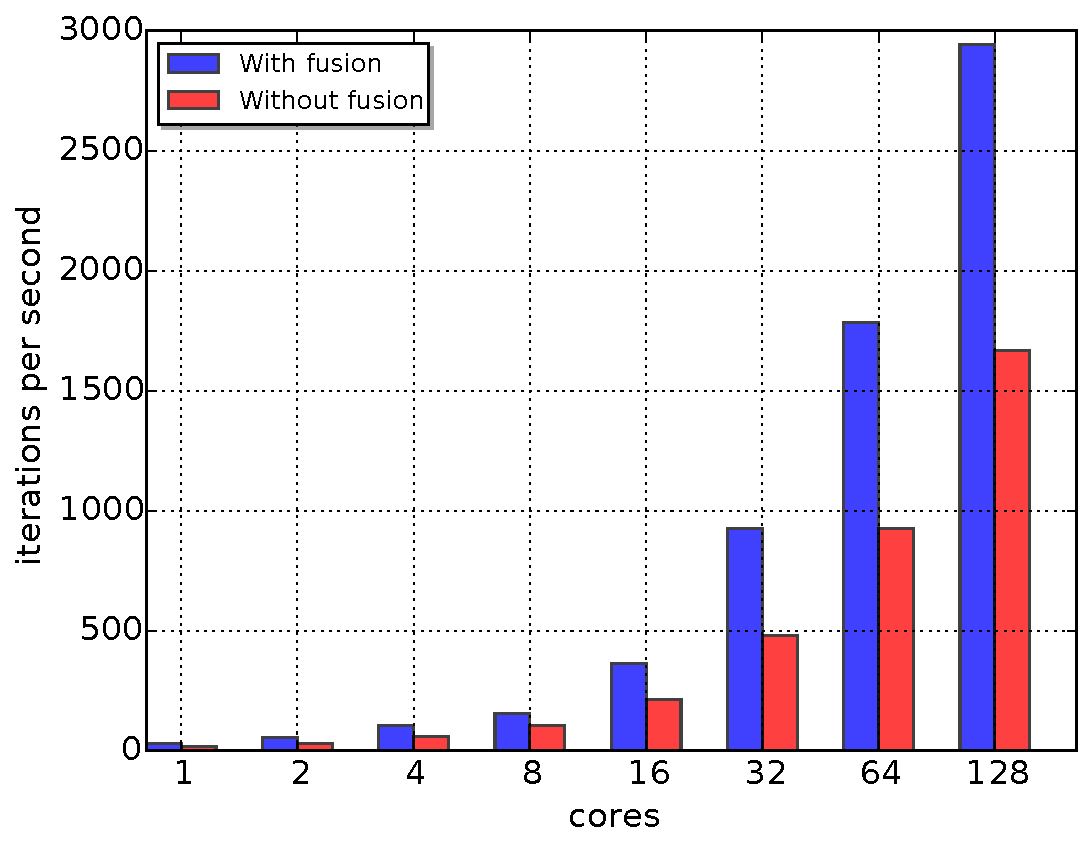
\includegraphics{../results/task_scaling/500_200/fusVSbase.pdf}}
  \caption{Strong scaling on a 500x500 domain, with and without the fusion optimization.}
  \label{fig:fusion}
\end{center}\end{figure}

%-------------------------------------
\subsection{Hybrid parallelism}

The series-parallel tree decomposition $TSP$ of this simulation, extracted by the MSL compiler, is composed of 17~sequence nodes and 18~parallel nodes. Table~\ref{fig:freq} represents the number of time a given level of parallelism, \ie the number of tasks to perform concurrently, is observed in the final tree. One can notice that the level of task parallelism extracted from the Shallow water equations is limited by two sequential parts in the application (level 1). Moreover, a level of 16~parallel tasks is reached two times, and five times for the fourth level.
This means that if two threads are dedicated to task parallelism, two parts of the code at least will not take advantage of this and that no part of the code would benefit from more than 16 threads.

\begin{table}[!h]
 \begin{center}
 \begin{tabular}{|c|c|c|c|c|c|c|c|c|}
    \hline 
   Level & 1 & 2 & 3 & 4 & 6 & 10 & 12 & 16\\
   \hline
   Frequency & 2 & 1 & 3 & 5 & 3 & 1 & 1 & 2\\
   \hline
 \end{tabular}
\caption{Parallelism level (number of parallel tasks) and the number of times this level appears.}
\label{fig:freq}
 \end{center}
\end{table}

The second parallelization technique proposed by MSL is an hybrid parallelization which mixes data parallelization and task parallelization. To implement this hybrid parallelization, the dump step of the MSL compiler uses the SkelGIS language, and the OpenMP language.

First, Figure~\ref{fig:limit} illustrates limitations of data parallelization technique alone. As explained in Section~\ref{sect:perfs}, performance of data parallelism is limited by the communication time between resources. As a result, when the size of sub-domain for each core becomes too small, and as the communication time increases with the number of cores, the strong speedup of the data parallelization starts to bend down. To catch this phenomena without too much cores, a relatively small domain of $500 \times 500$ is used.

\begin{figure}[!h]\begin{center}
  \resizebox{8cm}{!}{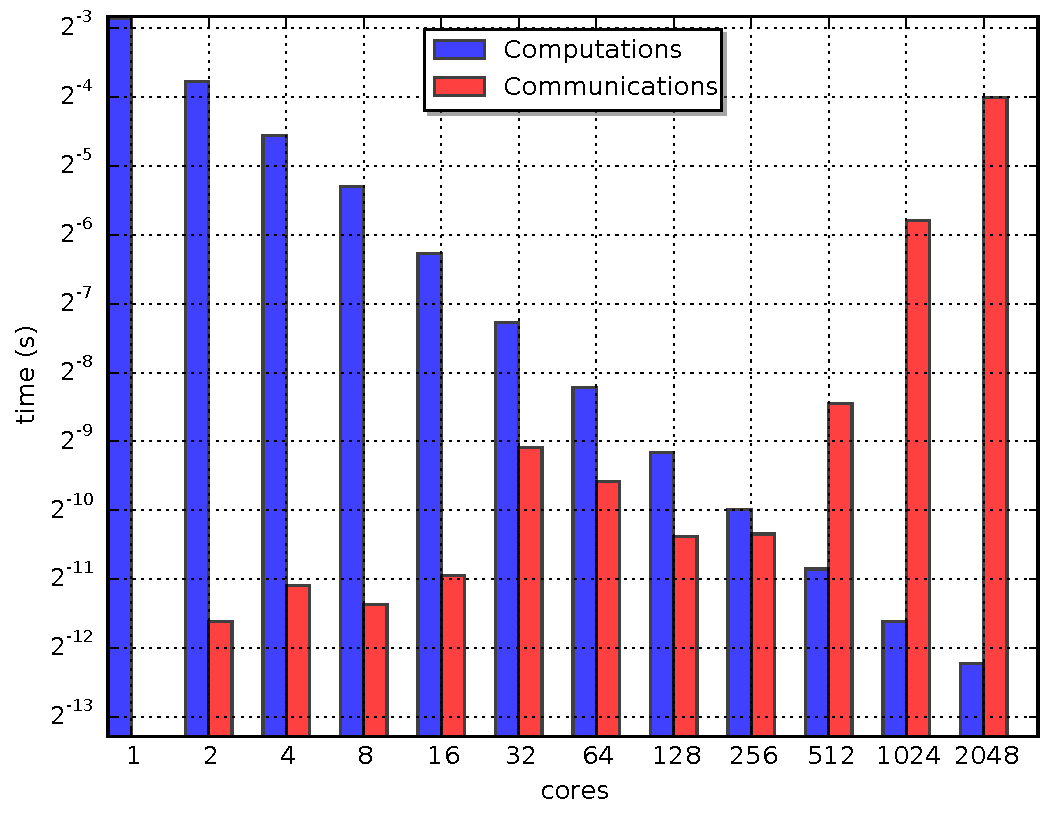
\includegraphics{../results/task_scaling/500_200/analytic/times.pdf}}
  \caption{Computation vs communication times in the data parallelization technique.}
  \label{fig:limit}
\end{center}\end{figure}

As expected, from 1 to 2048 cores the computation times decrease linearly. On the other hand, from 1 to 256 cores the communication time is almost constant, but from 256 to 2048 cores it increases. As a result from 512 cores to 2048 cores, the communication time becomes greater than the computation time. In Figure~\ref{fig:close}, the blue curve shows the strong scaling of the same example. Thus, from 256 to 2048 cores, the speedup bends down.

\medskip
In addition to the blue curve, Figure~\ref{fig:close} shows strong scalings for the same example but using an hybrid parallelization. For example, the purple curve shows the parallelization which uses 8 cores, to perform the task parallelization, for each process used for data parallelization (\ie MPI process). As a result, for example, when using 2 machines of the TGCC cluster, with a total of 32 cores, 4 cores are used for SkelGIS MPI processes, for data parallelization, and for each one 8 cores are used for task parallelization ($4 \times 8 = 32$).

As a result, and as explained in Section~\ref{sect:perfs}, data is less divided into sub-domains and the effect which is observe onto the blue curve is delayed. This figure shows a comparison with 2, 4, 8 and 16 cores per MPI process for task parallelization.

\begin{figure}[!h]\begin{center}
  \resizebox{8cm}{!}{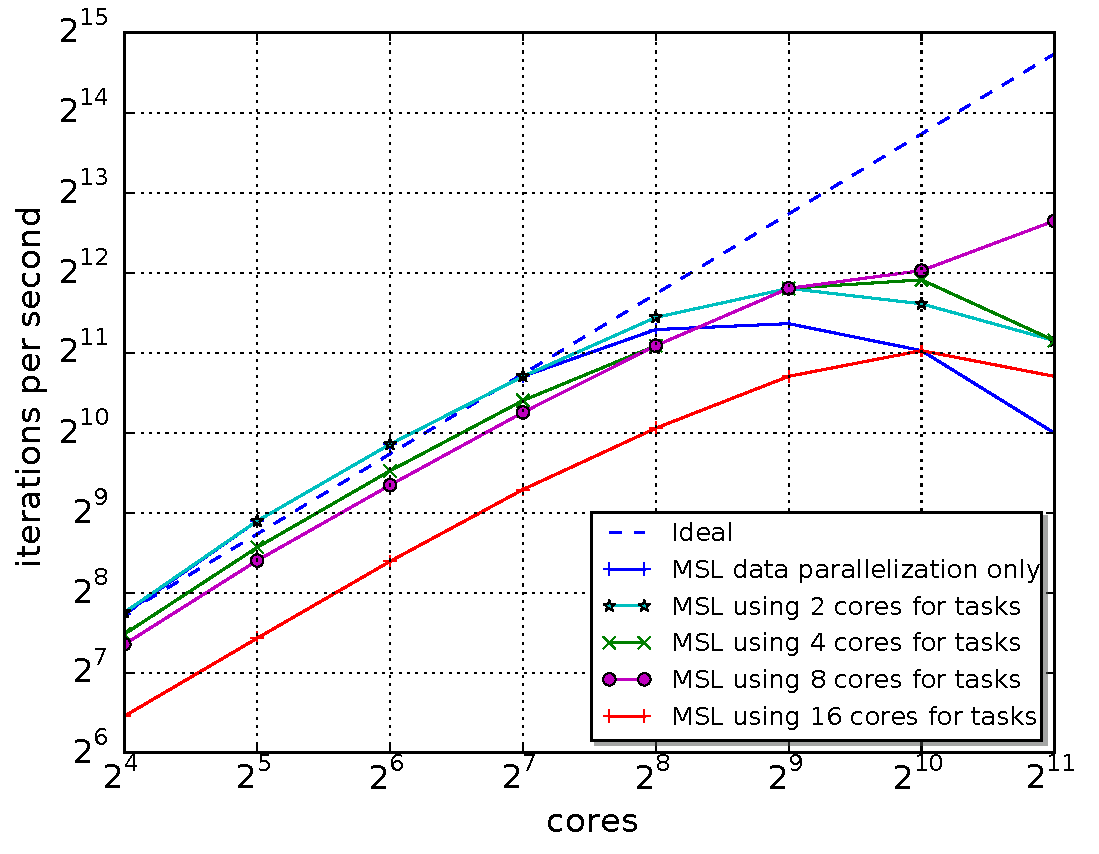
\includegraphics{../results/task_scaling/500_200/base_close_median.pdf}}
  \caption{Strong scaling comparisons between data parallelization and hybrid parallelization. A \emph{close} OpenMP clause is used to bind threads onto cores.}
  \label{fig:close}
\end{center}\end{figure}

From 2 to 8 cores, the improvement of the strong scaling is clear. However, reaching 16 cores, an important initial overhead appears and in addition to this, the curve bends down rapidly instead of improving the one with 8 cores for task parallelization. Two different phenomena happen.

First, thin nodes of the TGCC Curie are built with two NUMA nodes each of 8 cores. As a result, when increasing the number of OpenMP cores for task parallelization from 8 to 16 cores, an overhead is introduced by exchanges of data between memories of the two NUMA nodes. This phenomena is illutrated in Figure~\ref{fig:spread}. In this figure, a different strategy is used to bind threads onto available cores (using OpenMP). This strategy, called \emph{spread} instead of \emph{close} in Figure~\ref{fig:close}, binds threads on cores in order to spread as much as possible onto resources, which means that the two NUMA nodes are directly used whatever the number of cores kept for task parallelization. As a result, and as shown in the figure, using 2, 4 and 8 cores an initial overhead is introduced.

\begin{figure}[!h]\begin{center}
  \resizebox{8cm}{!}{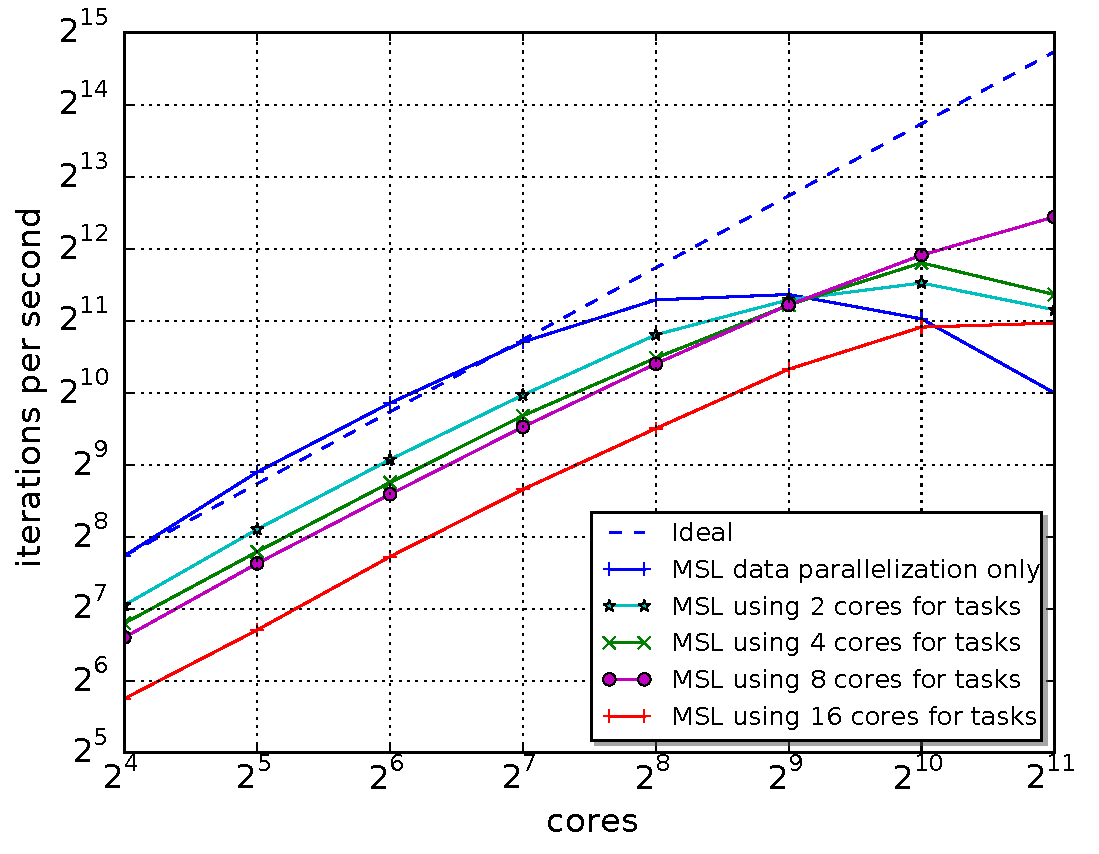
\includegraphics{../results/task_scaling/500_200/base_spread_median.pdf}}
  \caption{Strong scaling comparisons between data parallelization and hybrid parallelization. A \emph{spread} OpenMP clause is used to bind threads onto cores.}
  \label{fig:spread}
\end{center}\end{figure}

The second phenomena, which happens in Figure~\ref{fig:close} with 16 cores for tasks parallelization, is due to the level of parallelization introduced by the task parallelization technique. Actually, as illustrated in Table~\ref{fig:freq}, only two steps of the $TSP$ static scheduling generated by the MSL compiler can take advantage of 16 cores among a total of 18 steps. This phenomena has been explained in Section~\ref{sect:perfs} by the variable $F_{task}$ and the fact that it is not always true that $F_{task}=P_{task}$. This explains why using 16 cores for task parallelization in Figure~\ref{fig:spread} is still less efficient than using 8 cores even if the two NUMA nodes are always used in this evaluation.

Finally, to completely validate the performance model introduced in Section~\ref{sect:perfs}, and to understand when the hybrid parallelization becomes more interesting than the data parallelization, Figure~\ref{fig:tth2} represents $T_{COM1}$ and $T_{COM2}+T_{task}$ of Equation~(\ref{eq:hyb}), for the best case, \ie when 8 cores are used for task parallelization, and with a \emph{close} OpenMP bind of threads onto cores. Table~\ref{fig:tth} gives time details.

\begin{table}[!h]
 \begin{center}
 \begin{tabular}{|c|c|c|c|c|}
    \hline 
    & $T_{COM1}$ & $T_{COM2}$ & $T_{task}$ & Equation~(\ref{eq:hyb})\\
   \hline
   16 cores ($2 \times 8$) & 0.0005 & 0.00032 & 0.013 & False\\
   32 cores ($4 \times 8$) & 0.0018 & 0.00045 & 0.0062 & False\\
   64 cores ($8 \times 8$) & 0.0013 & 0.00038 & 0.0034 & False\\
   128 cores ($16 \times 8$) & 0.00075 & 0.0005 & 0.0023 & False\\
   256 cores ($32 \times 8$) & 0.00077 & 0.0018 & 0.001 & False\\
   512 cores ($64 \times 8$) & 0.0029 & 0.0013 & 0.00052 & True\\
   1024 cores ($128 \times 8$) & 0.018 & 0.00075 & 0.00029 & True\\
   2048 cores ($256 \times 8$) & 0.0623 & 0.00077 & 0.00016 & True\\
   \hline
 \end{tabular}
\caption{Execution times (seconds) of $T_{COM1}$, $T_{COM2}$ and $T_{task}$ for 8 cores for task parallelization. Verification of the Equation~(\ref{eq:hyb}).}
\label{fig:tth}
 \end{center}
\end{table}

\begin{figure}[!h]\begin{center}
  \resizebox{8cm}{!}{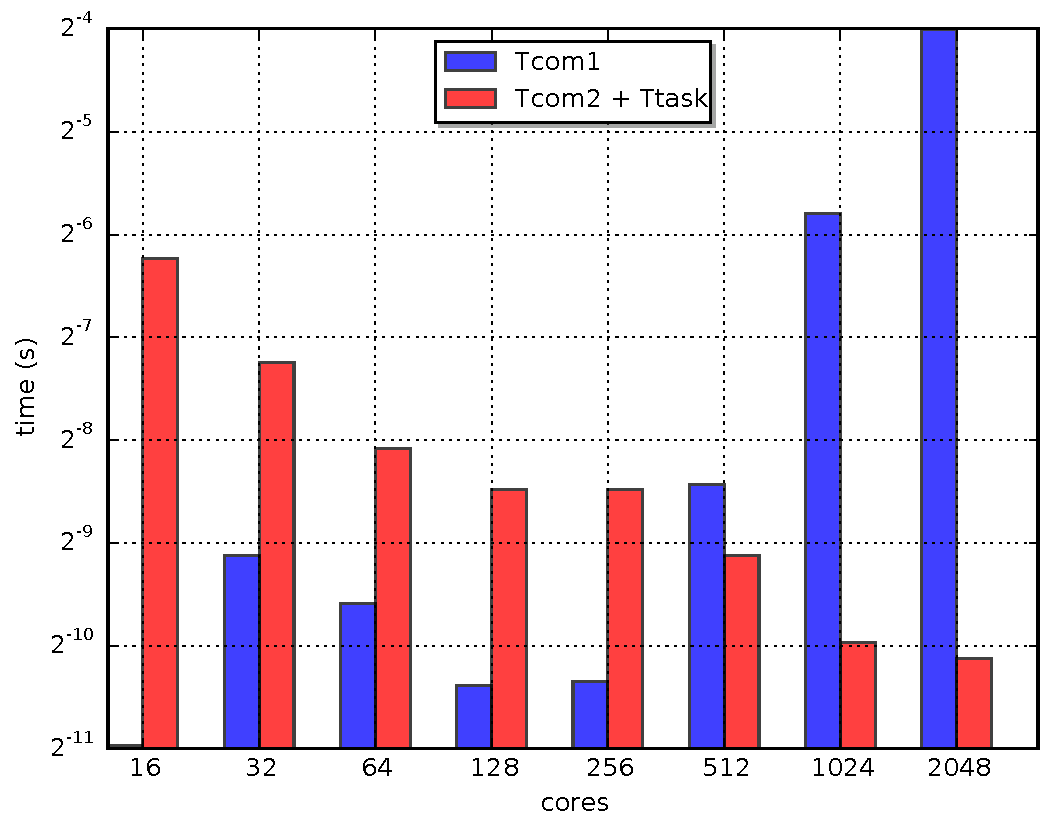
\includegraphics{../results/task_scaling/500_200/analytic/tth.pdf}}
  \caption{Execution times (seconds) of $T_{COM1}$ and $T_{COM2} + T_{task}$ for 8 cores for task parallelization. Verification of the Equation~(\ref{eq:hyb}).}
  \label{fig:tth2}
\end{center}\end{figure}

Figure~\ref{fig:tth2} and Table~\ref{fig:tth} perfectly matches results observed in Figure~\ref{fig:close} for 8 cores used for task parallelization per core used for data parallelization. As a result, the hybrid parallelization becomes better with a total of 512 cores.

%----------------------------------------
\section{Related Work}
\label{sect:related}
stencil compilation: Pochoir, PATUS etc.\\
stencil programs: Lizst, OP2\\
control in components: X-MAN (The New Component Model), STCM, Kell-calculus
%----------------------------------------
\section{Conclusion}
\label{sect:conclusion}
This paper has presented the domain specific language MSL and its compiler MSCAC designed to produce a parallel (data and hybrid) component-based runtime of an overall multi-stencil program, \ie a mesh-based numerical simulation reduced to explicit schemes. After details on the language and its compiler, MSL has been evaluated by the description of a real case numerical simulation: the shallow water equations. The component-based data parallelization of the simulation has been compared to a pure SkelGIS parallelization, and has shown improved execution times as well as a promising scalability. Those results demonstrate that component-based runtimes may be relevant back-end codes for DSLs as they do not introduce performance damage. Moreover, components bring software engineering benefits such as separation of concerns, code re-use, improving maintainability.

Although MSL is a promising case study from DSLs to component-based runtimes, many works in progress aims at improving this first contribution. First, to more clearly show the improvement of DSLs maintainability using component-based back-end, an alternative \texttt{DDS} component is under study, using Global Arrays~\cite{Nieplocha:2006:AAP:1125980.1125985}. In addition to this, alternatives for the \texttt{Computations} component, computed by MSC, are under study such as a dump to a pure OpenMP~\cite{660313} code or the use of dynamic schedulers~\cite{Augonnet2011,Gautier:2013:XRS:2510661.2511383}. %This last work on dynamic schedulers could also improve the expressivity of task parallelism in MSL, as discussed in Section~\ref{sect:eval}. Thus, it could bring interesting performance for the hybrid parallelization.

%----------------------------------------

\section{Acknowledgments}

Experiments presented in this paper were carried out using the
Grid'5000 testbed, supported by a scientific interest group hosted by
Inria and including CNRS, RENATER and several Universities as well as
other organizations (see \url{https://www.grid5000.fr}).

\small
\bibliographystyle{abbrv}
\bibliography{biblio}  

\end{document}
